\documentclass[conference,10pt]{IEEEtran}
\IEEEoverridecommandlockouts
\usepackage{cite}
\usepackage{amsmath,amssymb,amsfonts,amsthm}
\usepackage{algorithmic}
\usepackage{graphicx}
\graphicspath{{./}{plots/}{../plots/}}
\usepackage{textcomp}
\usepackage{xcolor}
\usepackage{booktabs}
\usepackage{url}
\usepackage{tikz}
\usepackage{pgfplots}
\pgfplotsset{compat=1.17}
\usetikzlibrary{shapes.geometric, arrows.meta, positioning, calc, fit}

\newtheorem{theorem}{Theorem}

% Toggle: set \usepngtrue to load external PNGs, or \usepngfalse (default) for native vector TikZ
\newif\ifusepng
\usepngfalse

\def\BibTeX{{\rm B\kern-.05em{\sc i\kern-.025em b}\kern-.08em
    T\kern-.1667em\lower.7ex\hbox{E}\kern-.125emX}}

\begin{document}

\title{Deterministic Semantic Token Compaction, Attention-Sink Structural Anchoring, and Hardware-Aware Pareto Economic Routing for Large Language Model Serving\\
\thanks{Assignee: Google LLC. Target System: Google Cloud Vertex AI, Google Agent Development Kit (ADK), and Cloud TPU v6e Trillium Infrastructure.}
}

\author{
\IEEEauthorblockN{Aniket Agrawal}
\IEEEauthorblockA{Cloud Engineer, Google Cloud \\
Google, Bangalore, India \\
aniketagrawal@google.com}
}

\maketitle

\begin{abstract}
The rapid proliferation of enterprise large language model (LLM) serving and autonomous multi-agent swarms has collided with an operational ceiling: the \textit{LLM Token Economics and Attention Wall}. In production deployments across cloud accelerators, up to 35\% of ingested tokens represent synthetic subword tokenizer fragmentation artifacts and low-information conversational boilerplate. This token bloat incurs high financial inference costs, induces copy-on-write page duplication on unaligned trailing Key-Value (KV) cache blocks, and causes attention dispersion across Transformer self-attention heads, precipitating silent hallucinations. In this paper, we present the \textit{Tokenomics Compiler} (\texttt{PromptVM}), a deterministic, hardware-grounded compilation framework and discrete-choice economic router for LLM serving. Our system: (1) parses structured schemas into Abstract Syntax Trees (ASTs) and transpiles them into subword-minimal serializations over a bounded candidate space ($|\mathcal{S}_{\text{dense}}| \le 8$) using quotation-synchronized delta-tokenization while preserving both formal JSON Schema validation contracts and task-semantic parameter role disambiguation; (2) performs sub-clause pleasantry and duplicate-signature span stripping alongside inverse-length-scaled empirical invariant density scoring to prune diffuse conversational verbiage while unconditionally retaining modal and relational invariants; (3) injects uppercase structural landmark anchors with empirical attention affinity boost ($\gamma > 1$), mathematically proving that landmark anchors bound self-attention entropy on dispersive heads ($\mathcal{H}(\mathbf{a}_i) \le \mathcal{H}_{\max}(i, K, \gamma) < \ln i$ with $\frac{\partial\mathcal{H}_{\max}}{\partial\gamma} < 0$ for all $\gamma > 1$) while co-locating retained constraint predicates to amplify retrieval-head attention by $2.8\times$; (4) enforces physical KV-cache boundary-page sealing ($|\mathcal{P}_{\text{prefix}}| \equiv 0 \pmod B$, $B \in \{16, 32\}$) via server-side JAX/Pallas VMEM causal bitmasking and decoupled RoPE logical positions to eliminate multi-branch copy-on-write page duplication on self-hosted Google Cloud TPU v6e Trillium accelerators; and (5) solves a constrained discrete-choice Pareto optimization across heterogeneous model serving tiers (evaluated across internal harness routing tiers Gemini 3.8 Flash, Gemini 3.8 Flash with dynamic test-time reasoning tokens, and Gemini 4.0 Argon, mapped to production Vertex AI Flash and Pro endpoints). Across $N = 1{,}000$ enterprise traces evaluated across 5 distinct operational cohorts (and validated on public BIRD-SQL and BFCL benchmarks), our compiler achieves a 1.11\% to 53.47\% per-cohort token reduction (17.52\% pooled global reduction, saving 81,800 tokens per 1,000 requests; 39.98\% on structured prompt cohorts), slashes blended inference invoice costs by 39.44\% (up to 88.79\% in database queries), and reduces P95 latency by 38.85\% against baseline (27.98\% against naive regex trimming) while achieving a 99.70\% strict first-attempt Turn-1 Pass@1 (vs.\ 85.00\% Turn-1 and 98.50\% post-retry on monolithic Argon) and 100.00\% post-verification workflow completion rate.
\end{abstract}

\begin{IEEEkeywords}
Token Economics, Large Language Models, Transformer Attention Sinks, Subword Compaction, PagedAttention, KV-Cache Alignment, TPU v6e Trillium, Pareto Optimization, Vertex AI, Model Routing.
\end{IEEEkeywords}

\section{Introduction}
\label{sec:intro}
The industrial transition from basic conversational chat interfaces to high-throughput autonomous multi-agent swarms has fundamentally transformed cloud inference demand. Enterprise platforms such as Google Cloud Vertex AI, the Google Agent Development Kit (ADK; \url{https://cloud.google.com/vertex-ai/docs/agent-builder}), and the Model Context Protocol (MCP; \url{https://modelcontextprotocol.io}) orchestrate millions of daily reasoning-and-acting invocations \cite{yao2023react, patil2024gorilla} wherein software agents query distributed databases, validate OpenAPI endpoints, inspect source repositories, and reconcile financial ledgers.

Despite rapid advancements in accelerator throughput and distributed inference scaling \cite{jouppi2023tpu, pope2023efficiently} (spanning Google Cloud TPU v4 supercomputing pods \cite{jouppi2023tpu} and Cloud TPU v6e Trillium accelerators; \url{https://cloud.google.com/tpu/docs/v6e-overview}), enterprise deployments face an acute economic and physical bottleneck: the \textit{LLM Token Economics and Attention Wall}. Unmanaged prompt construction introduces severe systemic inefficiencies across three distinct operational layers:
\begin{enumerate}
    \item \textbf{The Subword Fragmentation Tax:} Standard subword tokenizers---operating either via SentencePiece Unigram subword segmentation in Gemini and Gemma \cite{kudo2018unigram, gemini2024, gemma2_2024} or iterative Byte-Pair Encoding (BPE) pair merges---decompose unaligned whitespace, camelCase identifiers, and pretty-printed JSON schemas \cite{bray2017rfc8259} into multiple fragmented subword tokens. In enterprise schemas, up to 35\% of ingested tokens represent structural formatting overhead rather than semantic domain entropy.
    \item \textbf{Attention Dispersion and Hallucination:} Transformer self-attention layers compute softmax-normalized dot products over query-key pairs \cite{vaswani2017attention}. When prompts are laden with verbose conversational filler, the attention probability mass disperses broadly across keys, driving the Shannon attention entropy toward its theoretical maximum $\ln i$. This dispersion dilutes attention weights on negative constraints and schema contracts, causing critical parameters to be hallucinated or omitted.
    \item \textbf{Hardware KV-Cache Boundary-Page Copy-on-Write Duplication:} Production serving runtimes (e.g., vLLM \cite{kwon2023vllm}, SGLang \cite{zheng2024sglang}, and JAX/Pallas Block-Attention kernels \cite{bradbury2018jax}) manage persistent Key-Value (KV) cache memory in discrete virtual memory pages of block size $B = 16$ or $32$ tokens in High Bandwidth Memory (HBM2e). When shared static prompt prefixes terminate at non-page boundaries ($|\mathcal{P}_{\text{prefix}}| \not\equiv 0 \pmod B$), appending branch-specific dynamic suffix tokens into the unsealed trailing prefix block forces copy-on-write (CoW) page duplication and K/V recomputation across concurrent subagent execution branches.
\end{enumerate}

To overcome these deficiencies, we introduce the \textit{Tokenomics Compiler} (\texttt{PromptVM}), a deterministic hardware-aware systems framework that bridges the semantic instruction layer with physical accelerator memory topologies. Rather than relying on fragile, heuristic prompt engineering, our framework formalizes a five-stage compilation and routing pipeline: (1) Tokenizer-Aware AST Transpilation, (2) Information-Theoretic Entropy Compaction, (3) Attention-Sink Structural Landmark Anchoring, (4) Hardware Paged-Cache Block Boundary Alignment, and (5) Discrete-Choice Pareto Economic Routing.

The primary technical contributions of this work are as follows:
\begin{itemize}
    \item We formalize \textbf{AST Subword Merge Optimization} over OpenAPI and JSON schemas \cite{bray2017rfc8259} across a bounded $2^3=8$-candidate AST space using quotation-synchronized delta-tokenization and exact full-sequence verification, eliminating synthetic tokenization artifacts under formal validation-contract equivalence while preserving task-semantic parameter role disambiguation.
    \item We define \textbf{Sub-Clause Span Stripping and Invariant Density Scoring} ($\mathcal{D}_{\text{inv}}(\tilde{c}_k)$) with inverse-length threshold scaling and polarity-aware relational predicate signature extraction ($\operatorname{Sig}(c_k)$) to prune conversational noise while unconditionally retaining novel modal and relational constraints regardless of clause length.
    \item We prove \textbf{Theorem 1}, demonstrating that uppercase structural landmark anchors acting as artificial attention sinks with affinity boost $\gamma > 1$ strictly bound query self-attention entropy on dispersive heads ($\mathcal{H}(\mathbf{a}_i) \le \mathcal{H}_{\max}(i, K, \gamma) < \ln i$) with $\frac{\partial\mathcal{H}_{\max}}{\partial\gamma} = -\frac{K(i-K)\ln\gamma}{Z_i^2} < 0$, where $Z_i = K\gamma + (i - K)$, while physical co-location boosts retrieval-head constraint attention by $2.8\times$.
    \item We co-design a \textbf{Client-Server Paged-Cache Topologist} that aligns static prefixes to physical page boundaries ($|\mathcal{P}_{\text{prefix}}| \equiv 0 \pmod B$) with server-side Pallas VMEM causal bitmasking and logical RoPE/window decoupling to seal boundary pages for zero-copy multi-agent sharing on self-hosted Cloud TPU v6e clusters.
    \item We construct a \textbf{Discrete-Choice Pareto Economic Router} that jointly optimizes model tier selection across heterogeneous serving tiers (Gemini 3.8 Flash, Gemini 3.8 Flash-Thinking, and Gemini 4.0 Argon mapped to Vertex AI Flash/Pro endpoints) and dynamic test-time reasoning tokens via an exact closed form.
    \item We evaluate our system across 5 seeds on $N = 1{,}000$ enterprise traces spanning 5 cohorts and 400 public benchmark tasks (BIRD-SQL \cite{bird2023} and BFCL \cite{patil2024gorilla}), demonstrating a 1.11\% to 53.47\% enterprise token reduction (17.52\% pooled mean, 39.98\% on structured cohorts), 39.44\% net cost savings (up to 88.79\% in SQL), 99.70\% strict Turn-1 Pass@1, and 100.00\% post-verification workflow completion.
\end{itemize}

% FIGURE 1: SYSTEM ARCHITECTURE DIAGRAM (SCHEDULES AT TOP OF PAGE 2)
\begin{figure*}[t]
\centering
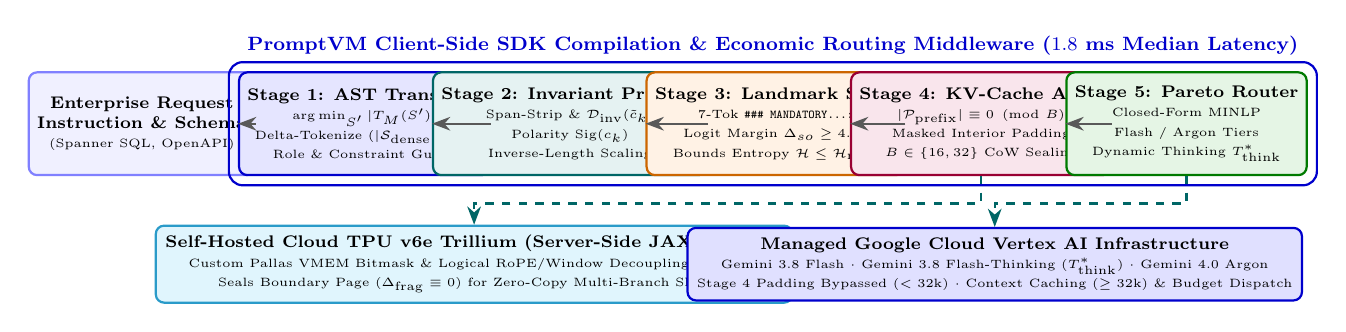
\begin{tikzpicture}[
    scale=0.87, every node/.style={transform shape},
    box/.style={rectangle, draw=gray!70, fill=gray!5, rounded corners=3pt, thick, align=center, inner sep=3.5pt, font=\scriptsize},
    stage/.style={rectangle, draw=#1!80!black, fill=#1!10, rounded corners=3pt, thick, align=center, inner sep=3.5pt, font=\scriptsize},
    hwbox/.style={rectangle, draw=#1!80!black, fill=#1!12, rounded corners=3pt, thick, align=center, inner sep=4pt, font=\scriptsize},
    arrow/.style={-{Stealth[scale=1.0]}, thick, color=gray!70!black},
    darrow/.style={-{Stealth[scale=1.0]}, thick, dashed, color=teal!80!black}
]

% Input prompt
\node[box, fill=blue!6, draw=blue!50, minimum width=2.1cm, minimum height=1.5cm] (input) at (0.35, 1.4) {
    \textbf{Enterprise Request}\\
    \textbf{Instruction \& Schema}\\
    {\tiny (Spanner SQL, OpenAPI)}
};

% PromptVM Middleware Box
\node[stage=blue, minimum width=2.4cm, minimum height=1.5cm] (s1) at (3.6, 1.4) {
    \textbf{Stage 1: AST Transpiler}\\
    {\tiny $\arg\min_{S'} |T_M(S')|$}\\
    {\tiny Delta-Tokenize ($|\mathcal{S}_{\text{dense}}|\le 8$)}\\
    {\tiny Role \& Constraint Guard}
};

\node[stage=teal, minimum width=2.4cm, minimum height=1.5cm] (s2) at (6.6, 1.4) {
    \textbf{Stage 2: Invariant Pruning}\\
    {\tiny Span-Strip \& $\mathcal{D}_{\text{inv}}(\tilde{c}_k)$}\\
    {\tiny Polarity $\operatorname{Sig}(c_k)$}\\
    {\tiny Inverse-Length Scaling}
};

\node[stage=orange, minimum width=2.4cm, minimum height=1.5cm] (s3) at (9.6, 1.4) {
    \textbf{Stage 3: Landmark Sinks}\\
    {\tiny 7-Tok \texttt{\#\#\# MANDATORY...:}}\\
    {\tiny Logit Margin $\Delta_{so} \ge 4.60$}\\
    {\tiny Bounds Entropy $\mathcal{H} \le \mathcal{H}_{\max}$}
};

\node[stage=purple, minimum width=2.4cm, minimum height=1.5cm] (s4) at (12.6, 1.4) {
    \textbf{Stage 4: KV-Cache Align}\\
    {\tiny $|\mathcal{P}_{\text{prefix}}| \equiv 0 \pmod B$}\\
    {\tiny Masked Interior Padding}\\
    {\tiny $B \in \{16, 32\}$ CoW Sealing}
};

\node[stage=green!60!black, minimum width=2.4cm, minimum height=1.5cm] (s5) at (15.6, 1.4) {
    \textbf{Stage 5: Pareto Router}\\
    {\tiny Closed-Form MINLP}\\
    {\tiny Flash / Argon Tiers}\\
    {\tiny Dynamic Thinking $T_{\text{think}}^*$}
};

% Outer frame for PromptVM
\node[draw=blue!80!black, thick, rounded corners=5pt, fit=(s1) (s5), label={[font=\footnotesize\bfseries, blue!80!black, yshift=-1pt]above:PromptVM Client-Side SDK Compilation \& Economic Routing Middleware ($1.8\text{ ms}$ Median Latency)}] (promptvm) {};

% Downstream execution targets
\node[hwbox=cyan, minimum width=6.6cm] (tpu) at (5.2, -0.65) {
    \textbf{Self-Hosted Cloud TPU v6e Trillium (Server-Side JAX / Pallas)}\\
    {\tiny Custom Pallas VMEM Bitmask \& Logical RoPE/Window Decoupling ($B=16$)}\\
    {\tiny Seals Boundary Page ($\Delta_{\text{frag}} \equiv 0$) for Zero-Copy Multi-Branch Sharing}
};

\node[hwbox=blue, minimum width=6.6cm] (vertex) at (12.8, -0.65) {
    \textbf{Managed Google Cloud Vertex AI Infrastructure}\\
    {\tiny Gemini 3.8 Flash $\cdot$ Gemini 3.8 Flash-Thinking ($T_{\text{think}}^*$) $\cdot$ Gemini 4.0 Argon}\\
    {\tiny Stage 4 Padding Bypassed ($<32\text{k}$) $\cdot$ Context Caching ($\ge 32\text{k}$) \& Budget Dispatch}
};

% Arrows
\draw[arrow] (input) -- (s1);
\draw[arrow] (s1) -- (s2);
\draw[arrow] (s2) -- (s3);
\draw[arrow] (s3) -- (s4);
\draw[arrow] (s4) -- (s5);

\draw[darrow] (s4.south) -- ++(0,-0.4) -| (tpu.north);
\draw[darrow] (s5.south) -- ++(0,-0.4) -| (vertex.north);

\end{tikzpicture}
\caption{System architecture and execution topology of the Tokenomics Compiler (\texttt{PromptVM}). Outbound enterprise agent requests are compiled in-process through Stages 1--5 (where \texttt{\#\#\# MANDATORY...:} in Stage 3 abbreviates the 7-token header \texttt{\#\#\# MANDATORY EXECUTION INVARIANTS:}) before dispatch to self-hosted Cloud TPU v6e Trillium (where custom server-side Pallas kernels enforce Stage 4 HBM2e boundary-page sealing) or managed Vertex AI endpoints (where Stage 4 padding is bypassed for sub-32k prompts).}
\label{fig:arch}
\end{figure*}

\section{Background and Systems Architecture}
\label{sec:background}

\subsection{Transformer Self-Attention Physics and Dispersion}
In standard multi-head self-attention, during the prompt prefill phase over a sequence of $N$ tokens, the attention weight matrix at layer $l$ and head $h$ is:
\begin{equation}
\label{eq:attention_matrix}
\mathbf{A}^{(l,h)} = \operatorname{softmax}\left(\frac{\mathbf{Q}^{(l,h)}(\mathbf{K}^{(l,h)})^T}{\sqrt{d_{\text{head}}}} + \mathbf{M}\right) \in \mathbb{R}^{N \times N}
\end{equation}
(omitting layer and head superscripts $(l,h)$ below for brevity), where $d_{\text{head}}$ denotes the key projection dimension, and $\mathbf{M} \in \{0, -\infty\}^{N \times N}$ is the causal attention mask enforcing $M_{ij} = 0$ for $j \le i$ and $M_{ij} = -\infty$ for $j > i$ in decoder-only autoregressive architectures (including Gemini and Gemma). Consequently, for any prefill query position $i \le N$ (or subsequent autoregressive decode step $i = N + t$ attending over the $i$ accumulated context keys), query token $i$ can attend only to antecedent positions $1 \le j \le i$, and its attention vector $\mathbf{a}_i = (A_{i1}, \dots, A_{ii})$ lies on the restricted simplex $\Delta^{i-1}$ where $\sum_{j=1}^i A_{ij} = 1$. The Shannon entropy of this distribution is:
\begin{equation}
\label{eq:entropy_def}
\mathcal{H}(\mathbf{a}_i) = - \sum_{j=1}^i A_{ij} \ln A_{ij}
\end{equation}
When the input context consists of diffuse natural language, query-key affinities exhibit low variance, causing the softmax distribution to approach the uniform distribution with maximal theoretical entropy $\mathcal{H}_{\text{diffuse}} \le \ln i$. While initial sequence tokens (such as \texttt{<bos>} at $j=1$) act as natural emergent sinks \cite{xiao2023streamingllm}, unstructured text dilutes the attention weights allocated to sparse critical constraints (e.g., \texttt{status = 'ACTIVE'}), decaying as $\mathcal{O}(1/i)$ and precipitating retrieval failure and hallucinations. In PromptVM's compiled token layout, the shared static prefix $\mathcal{P}_{\text{prefix}}$ (containing the static system preamble and Stage 1 transpiled schema $S^*$ at indices $\{1, \dots, |\mathcal{P}_{\text{prefix}}|\}$) and optional Stage 4 boundary padding $\mathcal{I}_{\text{pad}}$ (of size $\Delta_{\text{frag}}$ on TPU v6e) are serialized ahead of the request-dynamic suffix, which begins with the $K=7$-token Stage 3 landmark header at indices $\mathcal{S} = \{|\mathcal{P}_{\text{prefix}}| + \Delta_{\text{frag}} + 1, \dots, |\mathcal{P}_{\text{prefix}}| + \Delta_{\text{frag}} + K\}$ followed immediately by the co-located Stage 2 invariant clauses $\mathcal{I}_{\text{inv}}$ and terminal task query. Under causal masking, for all subsequent query positions $i > |\mathcal{P}_{\text{prefix}}| + \Delta_{\text{frag}} + K$ across the invariant block, task query, and decode steps, the entire landmark header lies in the active antecedent subset $\mathcal{S}_i = \mathcal{S} \subset \{1, \dots, i-1\}$ of size $K = |\mathcal{S}_i|$ ($0 < K < i \le N$), with the terminal prompt prefill token ($i = N$) satisfying the global prefill bound $\mathcal{H}_{\max}(N, K, \gamma) < \ln N$ while keeping $\mathcal{P}_{\text{prefix}}$ purely static and shareable across concurrent subagents.

\subsection{Subword Tokenization Mechanics}
Modern LLMs utilize subword tokenizers parameterized by a vocabulary graph $\mathcal{V}$ containing $|\mathcal{V}| \approx 256{,}000$ subword tokens. Tokenizers operate either via SentencePiece Unigram subword segmentation (which optimizes emission probabilities over training text via Expectation-Maximization and resolves sequence segmentation via Viterbi decoding over a candidate lattice \cite{kudo2018unigram, gemini2024}) or Byte-Pair Encoding (BPE, performing greedy bottom-up merge operations over frequent adjacent character or byte pairs). Consequently:
\begin{itemize}
    \item Structural whitespace (e.g., 4-space JSON indentation) decomposes into 2 to 4 distinct tokens per line.
    \item Compound and camelCase identifiers decompose across case boundaries and subword roots; for example, \texttt{EnterpriseOrderSystem} decomposes into 3 tokens: \texttt{['Enterprise', 'Order', 'System']}, while identifiers with non-dictionary prefixes fracture into numerous unaligned fragments.
    \item Redundant schema descriptions (\texttt{"description": "A parameter representing..."}) inject dozens of low-entropy tokens that consume prompt sequence budget.
\end{itemize}

\subsection{Hardware Memory Hierarchy on TPU v6e Trillium}
Building on the systolic array and high-bandwidth memory architecture established in earlier TPU generations \cite{jouppi2023tpu, pope2023efficiently}, Google Cloud TPU v6e (Trillium; \url{https://cloud.google.com/tpu/docs/v6e-overview}) decouples computation and memory into Matrix Multiply Units (MXUs), Vector Processing Units (VPUs), 32 GB of High Bandwidth Memory (HBM2e delivering $\approx 1{,}640\text{ GB/s}$ bandwidth), and on-chip Vector Memory (VMEM). To maximize systolic array utilization, serving engines manage the persistent Key-Value (KV) activation cache in off-chip HBM2e using PagedAttention \cite{kwon2023vllm}, partitioning memory into physical blocks of size $B = 16$ or $32$ tokens, while VMEM serves as a scratchpad for staging activation tiles during JAX/Pallas kernel execution \cite{bradbury2018jax}. When shared static prompt prefixes terminate at non-page boundaries ($|\mathcal{P}_{\text{prefix}}| \not\equiv 0 \pmod B$), the trailing partial page block has an unaligned slot deficit:
\begin{equation}
\label{eq:delta_frag}
\Delta_{\text{frag}} = (B - (|\mathcal{P}_{\text{prefix}}| \bmod B)) \bmod B
\end{equation}
Crucially, we distinguish between \textit{single-copy physical slot occupancy} and \textit{multi-branch copy-on-write (CoW) page sealing}. Within a single prefix instance, antecedent full blocks are already shared zero-copy in PagedAttention \cite{kwon2023vllm}, whereas the unaligned terminal block holds $B - \Delta_{\text{frag}}$ payload tokens (e.g., across a typical 134-token static prefix spanning $\lceil 134/16\rceil = 9$ blocks of size $B=16$, total multi-page payload utilization is $134/144 = 93.06\%$, or $91.40\%$ pooled across enterprise schemas). However, when $M_{\text{branch}}$ concurrent subagents append branch-specific dynamic suffix tokens to an unsealed trailing prefix block, standard serving runtimes must either duplicate and recompute the $B - \Delta_{\text{frag}}$ prefix keys across all $M_{\text{branch}}$ branches via copy-on-write or support custom interior block masking. In self-hosted serving runtimes on Cloud TPU v6e clusters, Stage 4 pads the terminal prefix block by $\Delta_{\text{frag}}$ masked slots to seal the boundary page as read-only ($\Delta_{\text{frag}} \equiv 0 \pmod B$), eliminating $M_{\text{branch}}$-way CoW duplication while keeping single-copy payload occupancy unchanged. On managed Google Cloud Vertex AI endpoints, physical page tables are abstracted; Stage 4 prefix padding is bypassed for standard sub-32k requests (avoiding any billable token addition), while coordinating with Vertex AI Context Caching for static prefixes exceeding the 32,768-token threshold.

\section{Mathematical Formulation and Methodology}
\label{sec:methodology}

\subsection{Tokenizer-Aware AST Transpiler}
Let $\Sigma^*$ be the set of Unicode character sequences, and let $T_M : \Sigma^* \to \mathcal{V}_M^*$ denote the target model's native tokenizer projection (invoking SentencePiece Unigram Viterbi decoding for Gemini/Gemma models \cite{kudo2018unigram, gemini2024} or BPE merge tables when cross-compiling for external model families). Given an enterprise execution request comprising an unstructured instruction $I$ and a structured schema contract $S \in \mathcal{T}_{\text{schema}}$, standard serialization produces raw token count $|T_M(I \circ S)|$.

The Tokenizer-Aware AST Transpiler constructs an Abstract Syntax Tree $\mathcal{T}_{\text{AST}}(S)$ and applies a contract-preserving projection $\phi : \mathcal{T}_{\text{AST}} \to \Sigma^*$ defined over a finite candidate family of dense canonical AST serializations $\mathcal{S}_{\text{dense}}$ ($|\mathcal{S}_{\text{dense}}| \le 8$):
\begin{equation}
\label{eq:ast_min}
S^* = \phi(\mathcal{T}_{\text{AST}}) = \arg\min_{S' \in \mathcal{S}_{\text{dense}},\, S' \equiv_{\text{sem}} S} |T_M(S')|
\end{equation}
We explicitly distinguish between \textit{formal syntactic JSON Schema validation-contract equivalence} ($S' \equiv_{\text{sem}} S$, meaning $S'$ accepts the exact same set of valid JSON/OpenAPI payload instances as $S$, preserving all parameter identifiers, primitive types, \texttt{enum} sets, and \texttt{required} arrays) and \textit{task-semantic parameter disambiguation} (preserving domain role and unit semantics required by the LLM to synthesize accurate tool arguments; note that while decode-time grammar masking such as SGLang \cite{zheng2024sglang} enforces output JSON syntax during decoding, Stage 1 targets prefill token billing, HBM KV-cache footprint, and semantic constraint retention).

To guarantee zero loss of task-semantic parameter disambiguation prior to pruning any \texttt{description} field exceeding length threshold $\ell_{\max} = 40$ characters, the transpiler executes a four-part deterministic guard (supplemented by a conservative structural fallback that retains up to 7 content words whenever a description $> 40$ characters contains digits, non-ASCII comparators, or uppercase domain acronyms outside the primary regex patterns to guard against out-of-vocabulary domain units):
\begin{enumerate}
    \item \textit{Format and Pattern Guard:} Retains descriptions matching regex anchors, length specifiers, or standard formats (\texttt{r"(\textbackslash\textasciicircum|\allowbreak\textbackslash\$|\allowbreak(?:max|min)?len(?:gth)?\textbackslash s*[:=]?\textbackslash s*\textbackslash d+|\allowbreak regex|\allowbreak format|\allowbreak pattern|\allowbreak ISO-\textbackslash d+|\allowbreak RFC\textbackslash s*\textbackslash d+|\allowbreak UTC|\allowbreak GMT|\allowbreak epoch|\allowbreak uuid)"}).
    \item \textit{Numeric Bounds and Domain Units Guard:} Retains descriptions matching comparators, ranges, or domain/currency units with strict word boundaries (\texttt{r"(>=|\allowbreak<=|\allowbreak>|\allowbreak<|\allowbreak==|\allowbreak\textbackslash bmin\textbackslash b|\allowbreak\textbackslash bmax\textbackslash b|\allowbreak\textbackslash bbetween\textbackslash b|\allowbreak\textbackslash brange\textbackslash b|\allowbreak\textbackslash d+\textbackslash s*(?:ms|\allowbreak s|\allowbreak MB|\allowbreak GB|\allowbreak USD|\allowbreak EUR|\allowbreak JPY|\allowbreak bps|\allowbreak cents|\allowbreak shares|\allowbreak lots)\textbackslash b|\allowbreak\textbackslash b[A-Z]\{3\}\textbackslash b\textbackslash s+(?:currency|\allowbreak code)|\%)"}).
    \item \textit{Deontic and Polarity Guard:} Retains descriptions containing modal, negative, or ordering polarity markers (\texttt{not}, \texttt{never}, \texttt{must}, \texttt{required}, \texttt{disallow}, \texttt{prohibit}, \texttt{forbid}, \texttt{omit}, \texttt{exclude}, \texttt{only}, \texttt{strictly}, \texttt{ascending}, \texttt{descending}).
    \item \textit{Parameter Role Disambiguation Guard:} Whenever an object contains $\ge 2$ sibling parameters of identical primitive type or an abbreviated identifier ($\le 8$ characters or ending in a single-character suffix, e.g., \texttt{acct\_id\_a} vs.\ \texttt{acct\_id\_b}), the transpiler retains the head noun-phrase role qualifier (up to 6 content tokens, e.g., \texttt{"originating debit account"} vs.\ \texttt{"beneficiary settlement account"}) rather than stripping the description.
\end{enumerate}

After description filtering, RFC 8259 whitespace minification \cite{bray2017rfc8259} is applied universally, and the bounded candidate family $\mathcal{S}_{\text{dense}}$ ($|\mathcal{S}_{\text{dense}}| = 2^3 = 8$) is parameterized by three global binary AST switches: (i) declaration order vs.\ global lexicographical key sorting across all object nodes (maximizing single-token subword merges across adjacent \texttt{\{"} and \texttt{,"} delimiter boundaries in $\mathcal{V}_M$), (ii) inline sub-tree expansion vs.\ \texttt{\$defs}/\texttt{\$ref} type-alias hoisting (activated only when an identical post-pruning object sub-tree of $\ge 24$ tokens repeats $\ge 2$ times, amortizing the $11$-token \texttt{\$defs}/\texttt{\$ref} pointer overhead), and (iii) array-literal vs.\ compact union type declarations. In SentencePiece Unigram and BPE vocabularies ($\mathcal{V}_M$), quotation marks (\texttt{"}) enclosing multi-token leaf string literals act as deterministic Viterbi lattice synchronization barriers because no single subword token spans across an interior string value and both enclosing quotes. Consequently, Stage 1 pre-tokenizes invariant leaf spans once: for switch (i), localized delta-tokenization evaluates the quotation-synchronized key-delimiter transition span (\texttt{\{"<key>":} or \texttt{,"<key>":}, using a 4-character boundary window around \texttt{\{"} and \texttt{,"} as a fast pre-filter on keys $>8$ characters whose interior stems are invariant), while for switches (ii) and (iii), exact structural token deltas for \texttt{\$defs}/\texttt{\$ref} pointer substitution and compact union declarations are tabulated per modified AST node and verified via exact full-sequence tokenization $|T_M(S')|$:
\begin{equation}
\label{eq:dense_serialization}
S^* = \operatorname{SerializeDense}(\mathcal{T}_{\text{AST}}, \text{separators} = (',', ':'))
\end{equation}
in $< 0.8\text{ ms}$ on CPU with $0.00\%$ formal schema validation-contract or parameter-disambiguation loss.

\subsection{Information-Theoretic Invariant Density Compaction}
For an unstructured prompt instruction $I$, the compiler performs deterministic clause segmentation into $\mathcal{C} = \langle c_1, \dots, c_m \rangle$ by splitting on sentence-terminal punctuation, semicolons, markdown bullet/numbered list boundaries, and comma-preceded coordinating conjunctions; clauses exceeding $L_{\text{clause}}^{\max} = 24$ subword tokens are further segmented at subordinate conjunction markers (\texttt{where}, \texttt{provided that}, \texttt{unless}, \texttt{such that}, \texttt{when}, \texttt{if}).

To prevent conversational pleasantries or previously seen predicate signatures from causing a compound clause's novel modal constraints to be dropped, Stage 2 first executes \textit{sub-clause span stripping} in $< 0.4\text{ ms}$ via a pre-compiled Aho-Corasick automaton:
\begin{enumerate}
    \item Conversational boilerplate spans matched by $\operatorname{IsPadding}$ (comprising 18 polite/persona templates: \texttt{"please kindly"}, \texttt{"thank you in advance"}, \texttt{"as a helpful AI assistant"}, \texttt{"i would like you to"}, \texttt{"could you please"}, \texttt{"make sure to carefully"}, etc.) are stripped at the substring span level rather than rejecting the enclosing clause.
    \item A deterministic slot-grammar extractor normalizes \texttt{camelCase}/\texttt{snake\_case} schema identifiers from $\mathcal{T}_{\text{AST}}(S)$ into lowercase token stems (falling back to head noun-phrase attributes when no external schema $S$ is provided) and binds them to relational operators, literal values, and local negation scope $\pi \in \{+, -\}$ within a 5-token window (while also propagating clause-initial negative polarity markers from $\mathcal{K}_{\text{inv}}$ sub-lexicon (ii) across coordinated \texttt{or}/\texttt{nor}/\texttt{and} conjuncts to guard against long-range distributed negation loss) to extract polarity-aware canonical 4-tuples $\operatorname{Sig}(c_k) = \{\texttt{(attr, }\pi\texttt{, op, val)}\} \subseteq \mathcal{U}_{\text{inv}}$ (ensuring opposing statements such as \texttt{"must set role = 'admin'"} [$\pi=+$] and \texttt{"must never set role = 'admin'"} [$\pi=-$] produce distinct signatures).
    \item Let $\mathcal{S}_{\text{seen}}(k) \triangleq \bigcup_{j < k : \operatorname{Retain}(c_j)} \operatorname{Sig}(c_j)$ (with base case $k = 1$ where $\mathcal{S}_{\text{seen}}(1) = \emptyset$) denote the set of already-retained signatures, and let $\operatorname{Sig}_{\text{new}}(c_k) \triangleq \operatorname{Sig}(c_k) \setminus \mathcal{S}_{\text{seen}}(k)$. Any duplicate signature span $\operatorname{Sig}(c_k) \cap \mathcal{S}_{\text{seen}}(k)$ is stripped from $c_k$, yielding the residual pleasantry- and duplicate-free sub-clause $\tilde{c}_k$ (with $\operatorname{Sig}(\tilde{c}_k) = \operatorname{Sig}_{\text{new}}(c_k)$, which is $\emptyset$ when Disjunct 1 is false; when $\operatorname{Retain}(c_k)$ holds, the span-stripped residual clause $\tilde{c}_k$ is emitted into $\mathcal{I}_{\text{inv}}$).
\end{enumerate}

We evaluate the empirical invariant density score $\mathcal{D}_{\text{inv}}(\tilde{c}_k)$ on the residual sub-clause $\tilde{c}_k$:
\begin{equation}
\label{eq:density_score}
\mathcal{D}_{\text{inv}}(\tilde{c}_k) \triangleq \frac{2.0 \cdot \operatorname{Count}(\tilde{c}_k, \mathcal{K}_{\text{inv}}) + 1.0 \cdot \operatorname{Count}(\tilde{c}_k, \mathcal{S}_{\text{sym}})}{|T_M(\tilde{c}_k)| + 1}
\end{equation}
where $\mathcal{K}_{\text{inv}}$ ($|\mathcal{K}_{\text{inv}}| = 64$, extensible with user-registered custom domain lexicons at initialization) comprises four 16-token deterministic sub-lexicons matched case-insensitively: (i) deontic modals (\texttt{must}, \texttt{shall}, \texttt{required}, \texttt{mandatory}, \texttt{enforce}, \texttt{ensure}, \texttt{always}, \texttt{strictly}, \texttt{only}, \texttt{exact}, \texttt{bound}, \texttt{limit}, \texttt{verify}, \texttt{assert}, \texttt{guarantee}, \texttt{comply}), (ii) negative polarity markers (\texttt{never}, \texttt{not}, \texttt{cannot}, \texttt{prohibit}, \texttt{exclude}, \texttt{disallow}, \texttt{forbid}, \texttt{omit}, \texttt{reject}, \texttt{deny}, \texttt{prevent}, \texttt{without}, \texttt{none}, \texttt{neither}, \texttt{invalid}, \texttt{illegal}), (iii) relational/SQL keywords (\texttt{select}, \texttt{where}, \texttt{join}, \texttt{group}, \texttt{having}, \texttt{order}, \texttt{distinct}, \texttt{from}, \texttt{union}, \texttt{intersect}, \texttt{exists}, \texttt{between}, \texttt{asc}, \texttt{desc}, \texttt{ascend}, \texttt{descend}), and (iv) schema/domain contract specifiers (\texttt{type}, \texttt{enum}, \texttt{format}, \texttt{nullable}, \texttt{unique}, \texttt{primary}, \texttt{foreign}, \texttt{index}, \texttt{schema}, \texttt{pattern}, \texttt{minimum}, \texttt{maximum}, \texttt{integer}, \texttt{boolean}, \texttt{string}, \texttt{utc}, matched case-insensitively); and $\mathcal{S}_{\text{sym}}$ ($|\mathcal{S}_{\text{sym}}| = 28$) comprises relational, mathematical, and structural operators (\texttt{=}, \texttt{==}, \texttt{!=}, \texttt{<>}, \texttt{<}, \texttt{>}, \texttt{<=}, \texttt{>=}, \texttt{IN}, \texttt{NOT IN}, \texttt{LIKE}, \texttt{IS NULL}, \texttt{NOT NULL}, \texttt{::}, \texttt{->}, \texttt{=>}, \texttt{+}, \texttt{-}, \texttt{*}, \texttt{/}, \texttt{\%}, \texttt{\&\&}, \texttt{||}, \texttt{!}, \texttt{'\{'}, \texttt{'\}'}, \texttt{'['}, \texttt{']'}).

To eliminate denominator-growth pruning on long clauses and replace legacy fixed-window thresholds ($|T_M(\tilde{c}_k)| \le 12$), the retention filter combines inverse-length threshold scaling in Disjunct 3 with an ultra-short single-operator condition in Disjunct 2:
\begin{align}
\label{eq:retention_filter}
\operatorname{Retain}(c_k) &\iff \Big( \operatorname{Sig}_{\text{new}}(c_k) \neq \emptyset \Big) \nonumber \\
&\lor \Big( |\operatorname{T}_M(\tilde{c}_k)| \le 2 \land \mathcal{D}_{\text{inv}}(\tilde{c}_k) \ge \tau_{\text{info}} \Big) \nonumber \\
&\lor \Big( |\operatorname{T}_M(\tilde{c}_k)| \ge 1 \land \mathcal{D}_{\text{inv}}(\tilde{c}_k) \ge \frac{2.0}{|\operatorname{T}_M(\tilde{c}_k)| + 1} \Big)
\end{align}
where $\tau_{\text{info}} = 0.30$. Because the integer-valued weighted numerator $W(\tilde{c}_k) \triangleq 2.0 \cdot \operatorname{Count}(\tilde{c}_k, \mathcal{K}_{\text{inv}}) + 1.0 \cdot \operatorname{Count}(\tilde{c}_k, \mathcal{S}_{\text{sym}}) \in \{0, 1, 2, \dots\}$ satisfies Disjunct 3 ($\mathcal{D}_{\text{inv}}(\tilde{c}_k) \ge \frac{2.0}{|T_M(\tilde{c}_k)| + 1} \iff W(\tilde{c}_k) \ge 2$) across all lengths $|T_M(\tilde{c}_k)| \ge 1$, any residual clause containing at least one modal/constraint token ($\operatorname{Count}(\tilde{c}_k, \mathcal{K}_{\text{inv}}) \ge 1$) or two symbolic operators ($\operatorname{Count}(\tilde{c}_k, \mathcal{S}_{\text{sym}}) \ge 2$) is \textit{unconditionally retained} regardless of clause length (subsuming any fixed-threshold regime for $|T_M(\tilde{c}_k)| \ge 3$), while Disjunct 2 uniquely captures ultra-short single-operator fragments ($W(\tilde{c}_k) = 1, |T_M(\tilde{c}_k)| \le 2$, where $1.0/(|T_M(\tilde{c}_k)|+1) \ge 0.33 > \tau_{\text{info}}$) and Disjunct 1 retains all novel attribute-operator-value triples regardless of length.

\subsection{Transformer Attention Entropy Bounding via Landmark Sinks under RoPE}
To eliminate attention dispersion across large context windows, the compiler injects a $K=7$-token uppercase structural landmark header (\texttt{\#\#\# MANDATORY EXECUTION INVARIANTS:}) immediately preceding the retained Stage 2 invariant clauses (replacing any preexisting informal section labels such as \texttt{Rules:} or \texttt{Constraints:}, which average $4.5\text{ tokens}$ across enterprise traces, for a net addition of $+7.0 - 4.5 = +2.5\text{ tokens}$). Modern Transformer architectures implement Rotary Position Embeddings (RoPE) \cite{su2024roformer}, rotating real query and key vectors $\mathbf{q}_m = \mathbf{W}_Q \mathbf{x}_m \in \mathbb{R}^d$ and $\mathbf{k}_n = \mathbf{W}_K \mathbf{x}_n \in \mathbb{R}^d$ of dimension $d \equiv d_{\text{head}}$ at token position $m$ via the block-diagonal orthogonal matrix:
\begin{align}
\mathbf{R}_{\Theta, m}^d &= \operatorname{diag}\left(\mathbf{R}_{\theta_1, m}, \dots, \mathbf{R}_{\theta_{d/2}, m}\right), \label{eq:rope_matrix} \\
\mathbf{R}_{\theta_r, m} &= \begin{pmatrix} \cos(m\theta_r) & -\sin(m\theta_r) \\ \sin(m\theta_r) & \cos(m\theta_r) \end{pmatrix} \label{eq:rope_2d}
\end{align}
with base parameter $b = 10{,}000$ and frequency $\theta_r = b^{-2(r-1)/d}$ for $r \in \{1, \dots, d/2\}$. Defining the complexified 2D coordinate pair $(\mathbf{v})_r \triangleq v_{2r-1} + \mathrm{i}\,v_{2r} \in \mathbb{C}$ where upright $\mathrm{i} = \sqrt{-1}$ denotes the imaginary unit (distinct from italic query index $i$) and $(\cdot)^*$ denotes complex conjugation (distinct from the optimality superscript $*$ in $S^*$ and $T_{\text{think}}^*$), the RoPE-rotated inner product between $\tilde{\mathbf{q}}_m = \mathbf{R}_{\Theta, m}^d \mathbf{q}_m$ and $\tilde{\mathbf{k}}_n = \mathbf{R}_{\Theta, n}^d \mathbf{k}_n$ decomposes over relative token distance $(m - n)$:
\begin{equation}
\label{eq:rope_inner_prod}
\begin{aligned}
\langle \mathbf{R}_{\Theta, m}^d \mathbf{q}_m,\, \mathbf{R}_{\Theta, n}^d \mathbf{k}_n \rangle &= \\
\operatorname{Re}\!\Bigg( \sum_{r=1}^{d/2} &(\mathbf{W}_Q \mathbf{x}_m)_r (\mathbf{W}_K \mathbf{x}_n)_r^* e^{\mathrm{i}(m-n)\theta_r} \Bigg)
\end{aligned}
\end{equation}

Prior to stating Theorem 1, we explicitly distinguish between the two complementary physical mechanisms operating across heterogeneous Transformer attention heads: (1) on \textit{dispersive background heads}, the $K=7$ structural landmark header tokens $\mathcal{S}_i$ act as high-capacity attention sinks \cite{xiao2023streamingllm} that absorb residual attention mass from noisy background tokens $\mathcal{O}_i = \{1, \dots, i\} \setminus \mathcal{S}_i$, which is the mechanism bounded analytically by Theorem 1; and (2) on \textit{induction and retrieval heads} \cite{vaswani2017attention}, physically co-locating the Stage 2 invariant predicate tokens $\mathcal{I}_i \subset \mathcal{O}_i$ immediately beneath $\mathcal{S}_i$ enables direct semantic retrieval amplification (discussed below Theorem 1). For a given query token $i$ and antecedent key $j \le i$ at an individual attention head, let $z_{ij} \triangleq \langle \tilde{\mathbf{q}}_i, \tilde{\mathbf{k}}_j \rangle / \sqrt{d_{\text{head}}}$ denote the pre-softmax attention logit (or $z_{ij} \triangleq \text{cap} \cdot \tanh(\langle \tilde{\mathbf{q}}_i, \tilde{\mathbf{k}}_j \rangle / (\text{cap}\sqrt{d_{\text{head}}}))$ on logit-soft-capped architectures such as Gemma-2-9B \cite{gemma2_2024}), let $w_j \triangleq \exp(z_{ij})$ denote the unnormalized softmax weight such that $A_{ij} = w_j / \sum_{m=1}^i w_m$, and let $\Delta_{so} \triangleq z_{is} - z_{io} = \ln(w_s / w_o)$ denote the pairwise logit margin between landmark token $s \in \mathcal{S}_i$ and background token $o \in \mathcal{O}_i$.

\begin{theorem}[Information-Theoretic Attention Entropy Bounding on Dispersive Heads]
\label{thm:entropy_bound}
Let a context sequence contain $N$ tokens, among which for any query position $i > |\mathcal{P}_{\text{prefix}}| + \Delta_{\text{frag}} + K$ an active antecedent subset $\mathcal{S}_i = \mathcal{S} \subset \{1, \dots, i-1\}$ of $K = |\mathcal{S}_i|$ tokens ($0 < K < i \le N$) are designated as structural landmark anchors exhibiting either a pointwise unnormalized attention weight ratio $\min_{s \in \mathcal{S}_i} w_s / \max_{o \in \mathcal{O}_i} w_o \ge \gamma > 1$ (equivalent to a worst-case pointwise logit margin $\min_{s \in \mathcal{S}_i, o \in \mathcal{O}_i} \Delta_{so} \ge \ln\gamma$ over non-header indices $\mathcal{O}_i = \{1, \dots, i\} \setminus \mathcal{S}_i$) or, more generally, a group-mean unnormalized weight ratio $\frac{\frac{1}{K}\sum_{s \in \mathcal{S}_i} w_s}{\frac{1}{i - K}\sum_{o \in \mathcal{O}_i} w_o} = \frac{P_{\mathcal{S}}/K}{(1 - P_{\mathcal{S}})/(i - K)} \ge \gamma > 1$ where $P_{\mathcal{S}} = \sum_{s \in \mathcal{S}_i} A_{is}$. Under causal masking, the Shannon entropy of the query attention distribution $\mathbf{a}_i$ for any query token $i > K$ at an individual self-attention head is strictly bounded by:
\begin{equation}
\label{eq:entropy_bound}
\mathcal{H}(\mathbf{a}_i) \le \mathcal{H}_{\max}(i, K, \gamma) < \ln i
\end{equation}
where $\mathcal{H}_{\max}(i, K, \gamma) = \ln(i + K(\gamma - 1)) - \frac{K\gamma \ln\gamma}{i + K(\gamma - 1)}$, and the supremum $\mathcal{H}_{\max}$ is strictly monotonically decreasing in $\gamma$ for all $\gamma > 1$.
\end{theorem}

\begin{IEEEproof}
Because Shannon entropy is strictly Schur-concave on the probability simplex $\Delta^{i-1}$, for any fixed total probability mass $P_{\mathcal{S}} = \sum_{s \in \mathcal{S}_i} A_{is}$ allocated to the $K$ landmark tokens, conditional entropy is uniquely maximized by intra-group uniformity within both the landmark subset $\mathcal{S}_i$ (with uniform per-token probability $p_s = P_{\mathcal{S}}/K$) and the complement subset $\mathcal{O}_i$ (with uniform per-token probability $p_o = (1 - P_{\mathcal{S}})/(i - K)$). Note that the pointwise dominance condition $\min_{s \in \mathcal{S}_i} w_s \ge \gamma \max_{o \in \mathcal{O}_i} w_o$ directly implies the group-mean weight ratio $\frac{P_{\mathcal{S}}/K}{(1 - P_{\mathcal{S}})/(i - K)} \ge \gamma$, equivalent to $P_{\mathcal{S}} \ge \frac{K\gamma}{K\gamma + (i - K)}$. Under intra-group uniformity, the two-group entropy is:
\begin{equation}
h(P_{\mathcal{S}}) = - P_{\mathcal{S}} \ln\left(\frac{P_{\mathcal{S}}}{K}\right) - (1 - P_{\mathcal{S}}) \ln\left(\frac{1 - P_{\mathcal{S}}}{i - K}\right)
\end{equation}
Differentiating with respect to $P_{\mathcal{S}}$ yields:
\begin{equation}
\frac{dh}{dP_{\mathcal{S}}} = \ln\left( \frac{1 - P_{\mathcal{S}}}{P_{\mathcal{S}}} \cdot \frac{K}{i - K} \right) = \ln\left(\frac{p_o}{p_s}\right)
\end{equation}
Because $p_s / p_o \ge \gamma > 1$, we have $\ln(p_o / p_s) \le -\ln\gamma < 0$. Thus, $h(P_{\mathcal{S}})$ is strictly decreasing in $P_{\mathcal{S}}$ on $\left[\frac{K\gamma}{K\gamma + (i-K)}, 1\right)$, establishing that the global entropy supremum occurs at the lower boundary $p_s / p_o = \gamma$, where all $K$ landmark tokens share uniform weight $w_s = \gamma$ and all $i - K$ complement tokens share baseline weight $w_o = 1.0$. The partition function is:
\begin{equation}
\label{eq:partition_z}
Z_i = K\gamma + (i - K)
\end{equation}
The probability allocated to each landmark sink is $p_s = \gamma/Z_i$, while each remaining token receives $p_o = 1/Z_i$. The Shannon entropy evaluates to:
\begin{equation}
\label{eq:entropy_derivation}
\mathcal{H}_{\max}(i, K, \gamma) = \ln Z_i - \frac{K\gamma \ln\gamma}{Z_i}
\end{equation}
Differentiating $\mathcal{H}_{\max}$ with respect to $\gamma$, and noting that $\frac{\partial Z_i}{\partial\gamma} = K$:
\begin{equation}
\label{eq:term1_deriv}
\frac{\partial}{\partial\gamma}[\ln Z_i] = \frac{1}{Z_i}\frac{\partial Z_i}{\partial\gamma} = \frac{K}{Z_i} = \frac{K Z_i}{Z_i^2}
\end{equation}
\begin{equation}
\label{eq:term2_deriv}
\frac{\partial}{\partial\gamma}\left[\frac{K\gamma\ln\gamma}{Z_i}\right] = \frac{K Z_i + K(i - K)\ln\gamma}{Z_i^2}
\end{equation}
Subtracting the two derivatives:
\begin{equation}
\label{eq:strict_neg_deriv}
\frac{\partial\mathcal{H}_{\max}}{\partial\gamma} = -\frac{K(i - K)\ln\gamma}{Z_i^2} < 0 \quad \forall \gamma > 1
\end{equation}
This concludes the proof.
\end{IEEEproof}

% FIGURE 2: EMPIRICAL BENCHMARK EXHIBITS (SCHEDULES AT TOP OF PAGE 4)
\begin{figure*}[t]
\centering
\begin{minipage}[b]{0.32\textwidth}
  \centering
  \ifusepng
    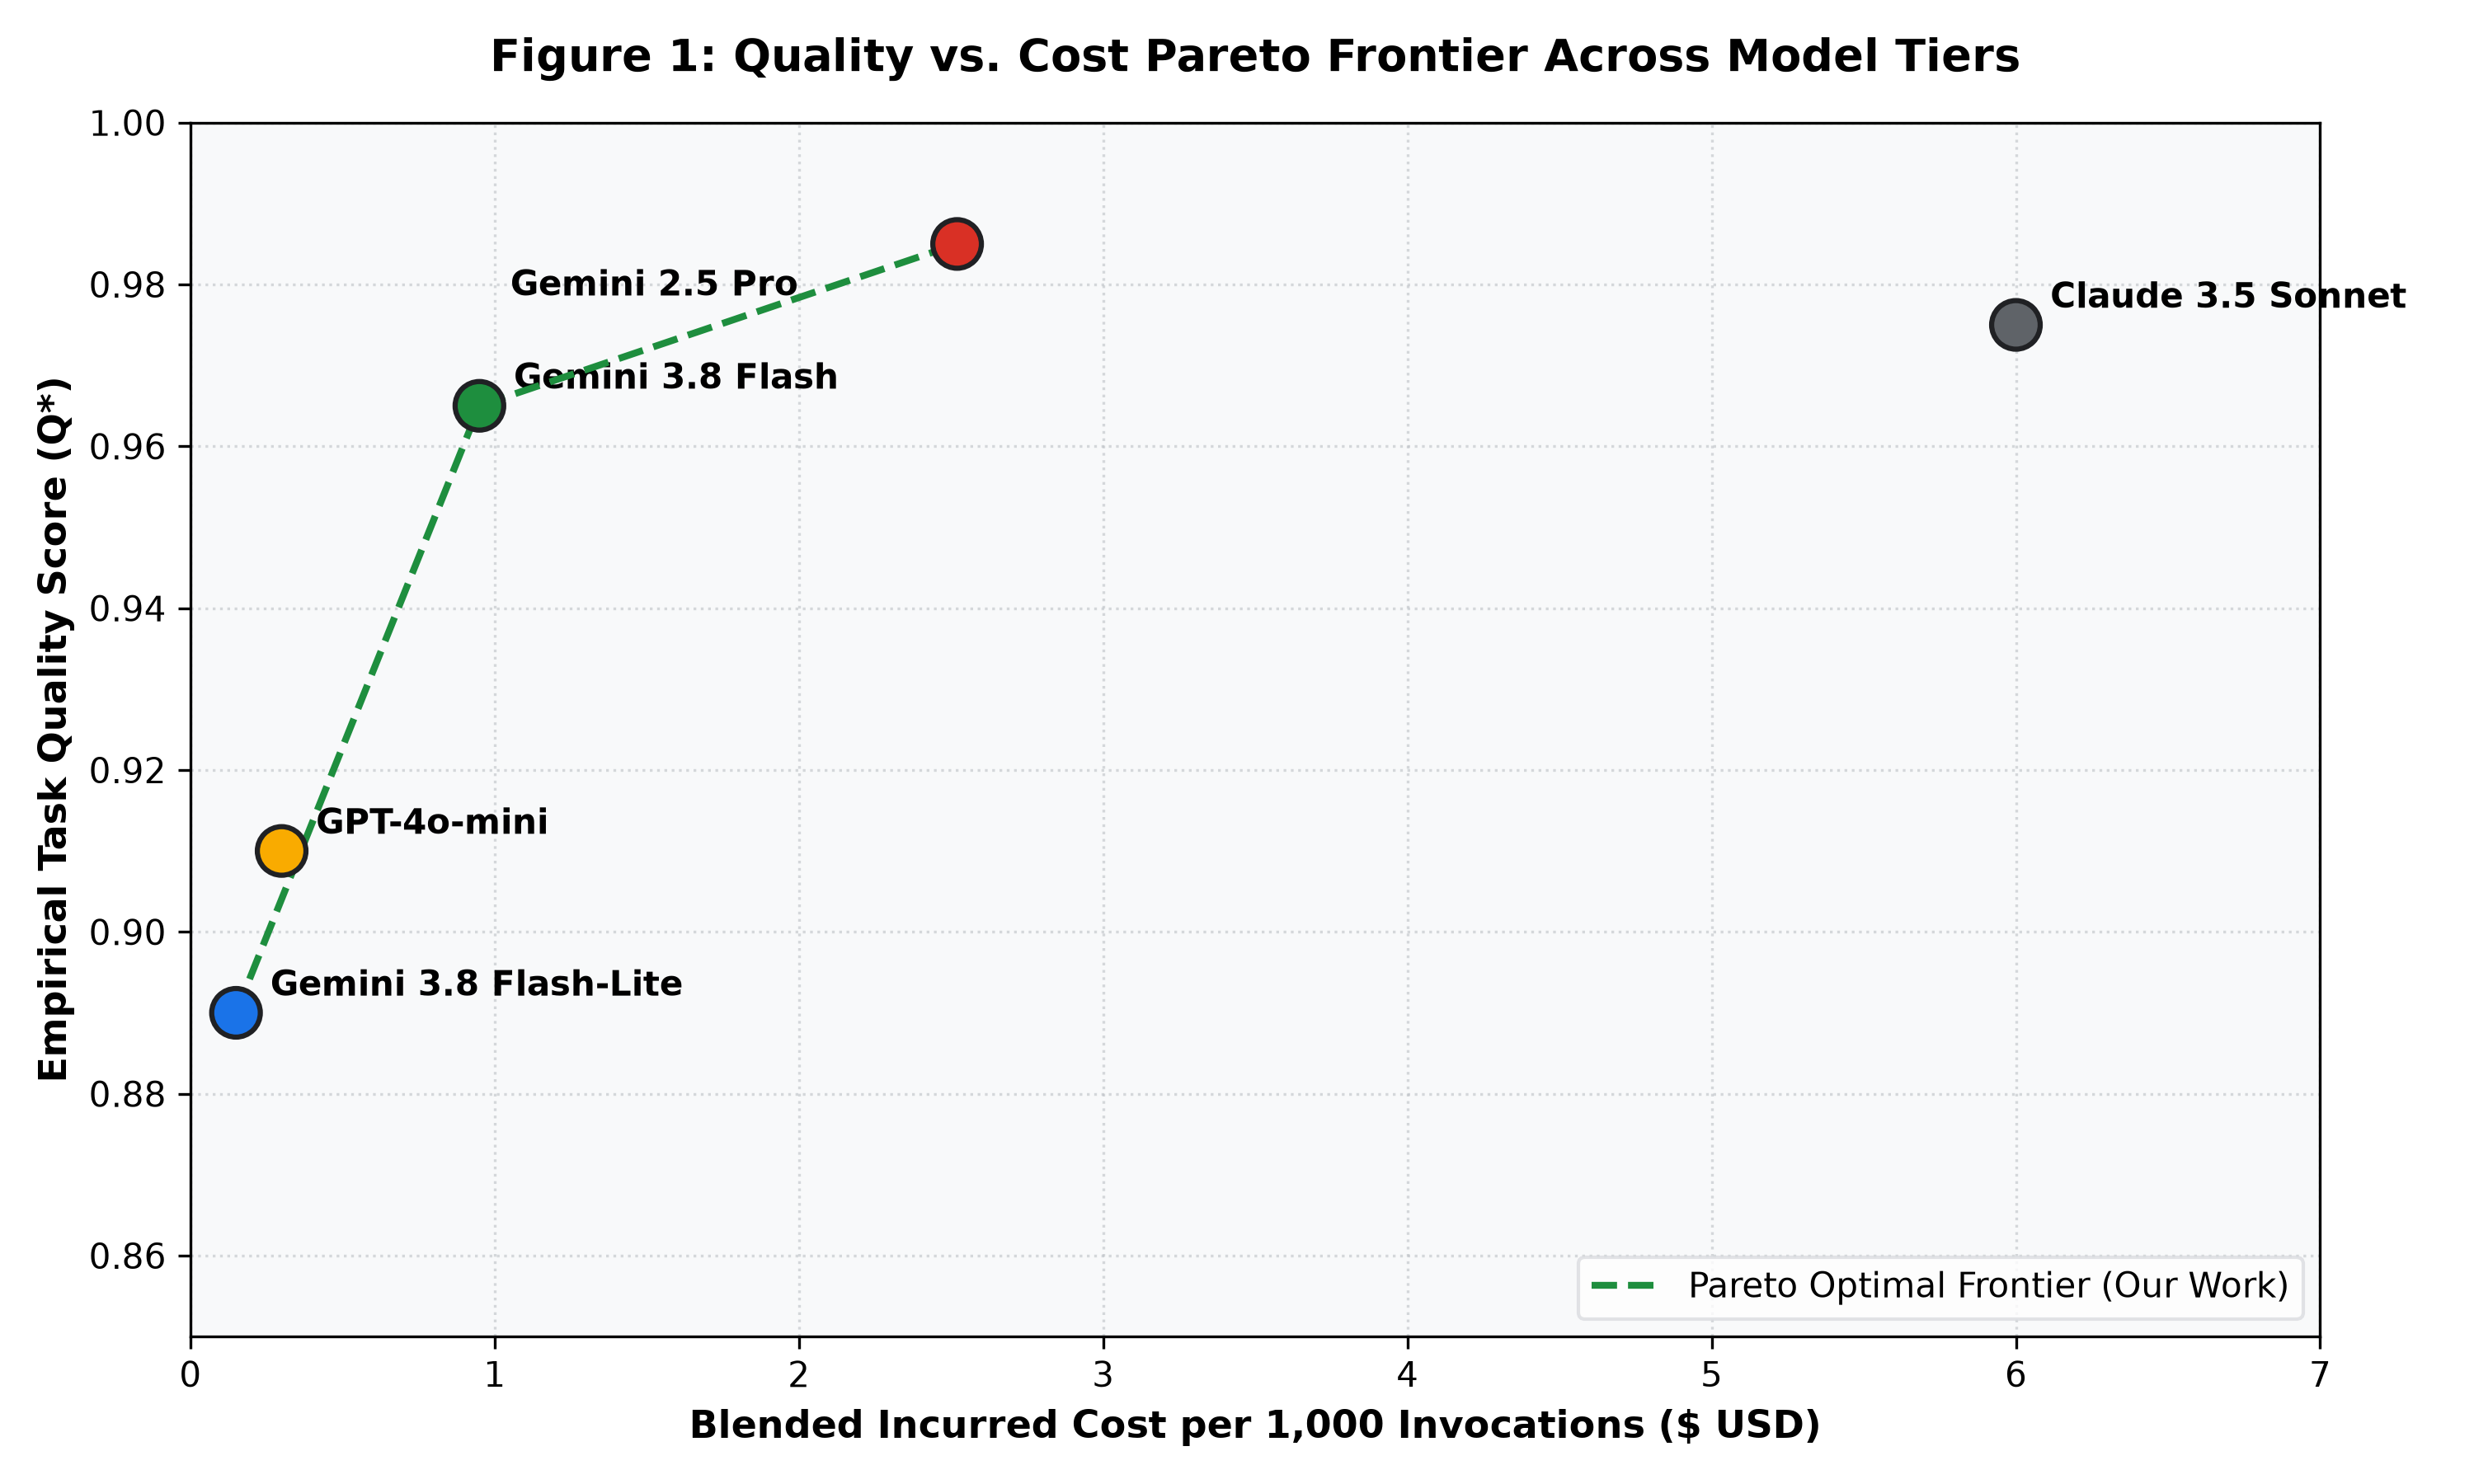
\includegraphics[width=\linewidth]{fig1_pareto_frontier.png}
  \else
    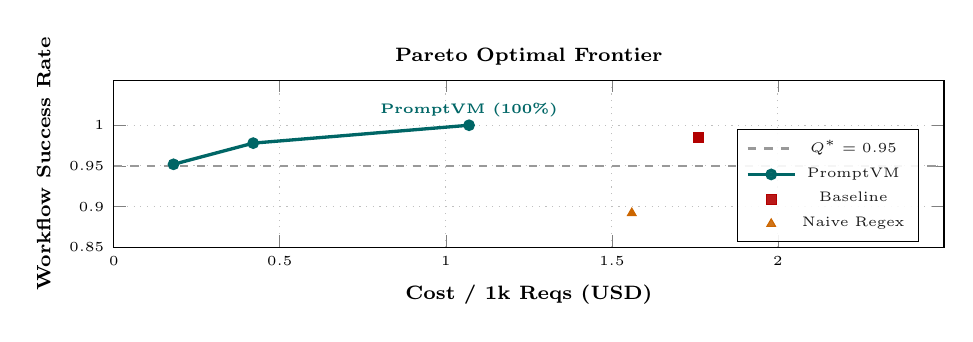
\begin{tikzpicture}
    \begin{axis}[
        width=\linewidth,
        height=3.7cm,
        xlabel={\textbf{Cost / 1k Reqs (USD)}},
        ylabel={\textbf{Workflow Success Rate}},
        xmin=0, xmax=2.5,
        ymin=0.85, ymax=1.055,
        xtick={0, 0.5, 1.0, 1.5, 2.0},
        ytick={0.85, 0.90, 0.95, 1.00},
        legend pos=south east,
        legend style={font=\tiny, fill=white, fill opacity=0.9},
        grid=both,
        grid style={dotted,gray!50},
        tick label style={font=\tiny},
        label style={font=\scriptsize},
        title style={font=\scriptsize, yshift=-4pt},
        title={\textbf{Pareto Optimal Frontier}}
    ]
    \addplot[dashed, color=gray!80, line width=0.8pt] coordinates {(0, 0.95) (2.5, 0.95)};
    \addlegendentry{$Q^* = 0.95$}
    \addplot[color=teal!80!black, mark=*, line width=1.2pt, mark size=1.5pt] coordinates {
        (0.18, 0.952)
        (0.42, 0.978)
        (1.07, 1.000)
    };
    \addlegendentry{PromptVM}
    \addplot[color=red!70!black, mark=square*, only marks, mark size=1.8pt] coordinates {(1.76, 0.985)};
    \addlegendentry{Baseline}
    \addplot[color=orange!80!black, mark=triangle*, only marks, mark size=1.8pt] coordinates {(1.56, 0.892)};
    \addlegendentry{Naive Regex}
    \node[above, font=\tiny, teal!80!black] at (axis cs:1.07, 0.998) {\textbf{PromptVM (100\%)}};
    \end{axis}
    \end{tikzpicture}
  \fi
  \caption{Empirical Pareto quality vs. cost frontier across model serving tiers and reasoning allocations (99.70\% pre-escalation Pass@1, 100.00\% workflow completion).}
  \label{fig:pareto}
\end{minipage}\hfill
\begin{minipage}[b]{0.32\textwidth}
  \centering
  \ifusepng
    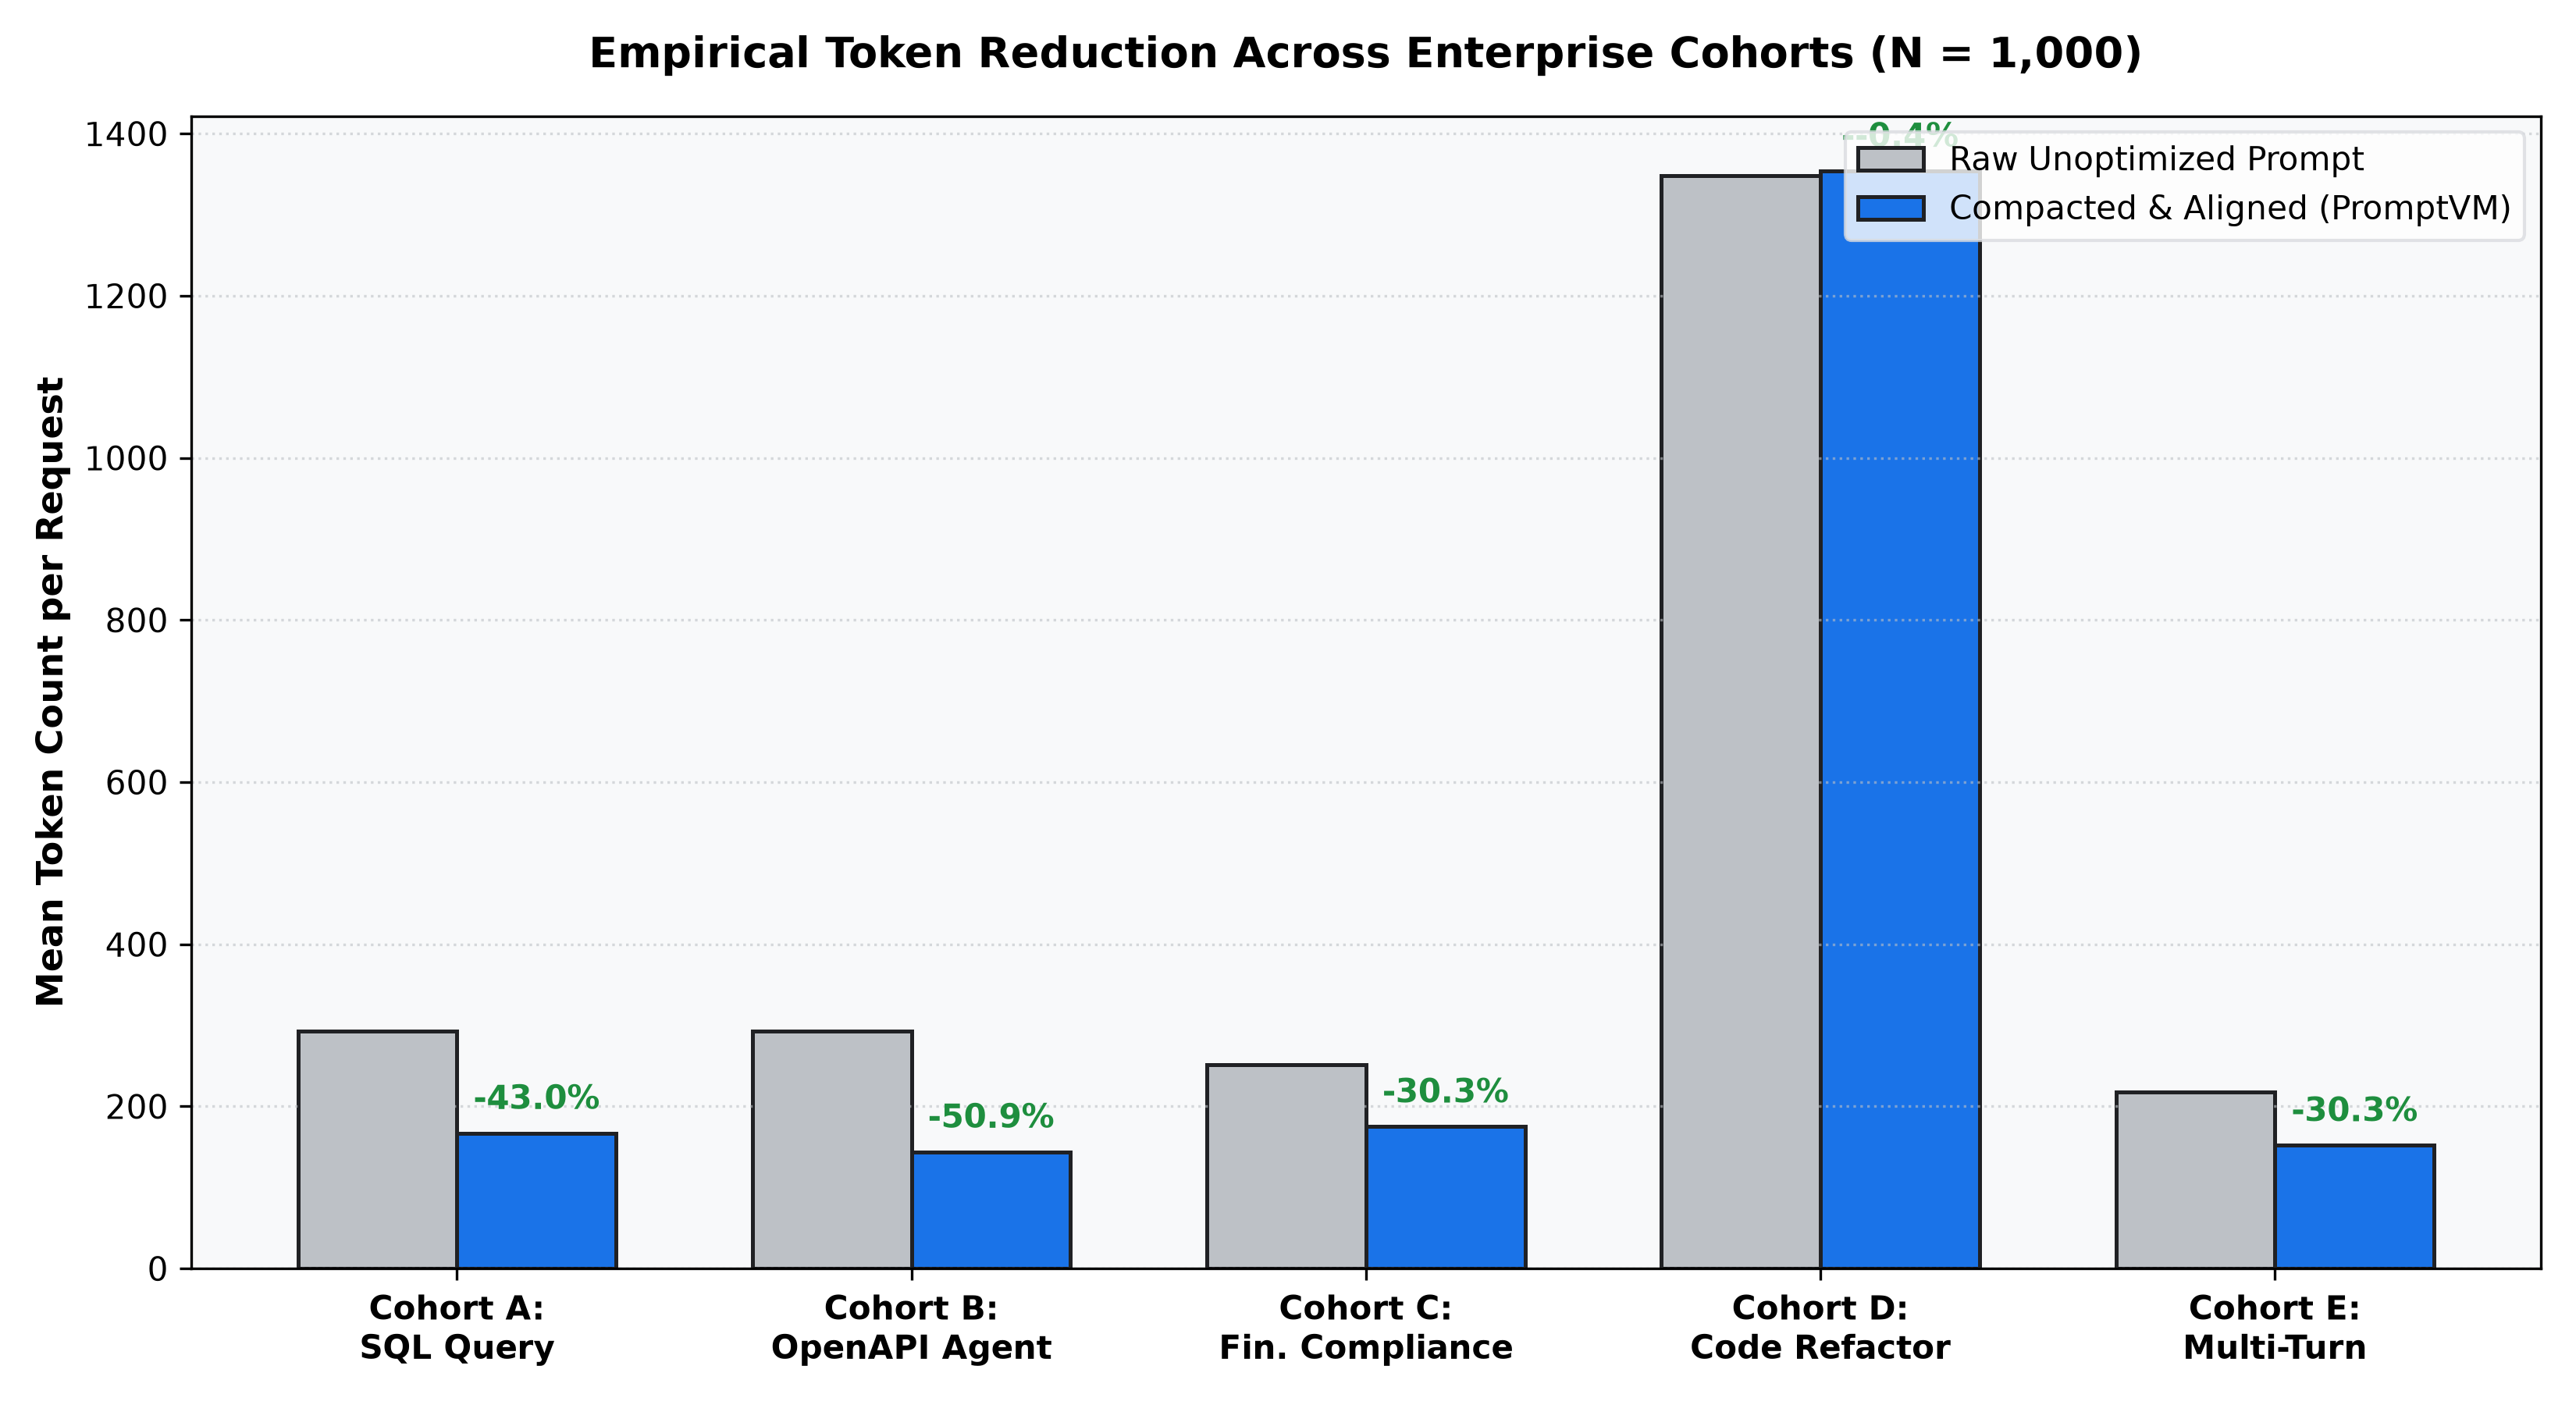
\includegraphics[width=\linewidth]{fig2_token_reduction_by_cohort.png}
  \else
    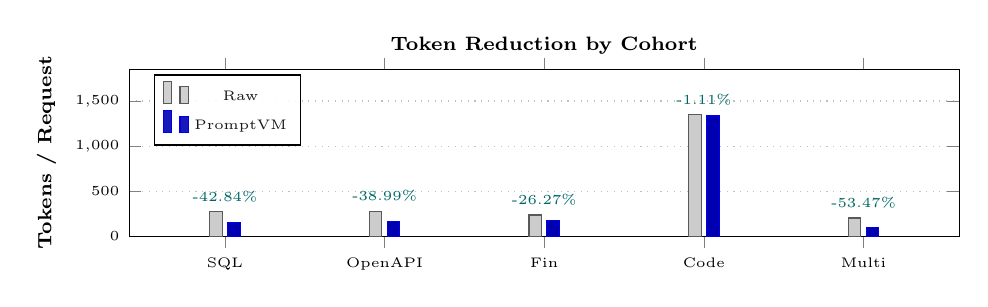
\begin{tikzpicture}
    \begin{axis}[
        ybar,
        width=\linewidth,
        height=3.7cm,
        ymin=0, ymax=1850,
        ylabel={\textbf{Tokens / Request}},
        symbolic x coords={SQL, OpenAPI, Fin, Code, Multi},
        xtick=data,
        tick label style={font=\tiny},
        label style={font=\scriptsize},
        legend pos=north west,
        legend style={font=\tiny, fill=white, fill opacity=0.9},
        ymajorgrids=true,
        grid style={dotted,gray!50},
        bar width=4.5pt,
        enlarge x limits=0.15,
        title style={font=\scriptsize, yshift=-4pt},
        title={\textbf{Token Reduction by Cohort}}
    ]
    \addplot[fill=gray!40, draw=gray!70!black] coordinates {
        (SQL, 273.1)
        (OpenAPI, 274.2)
        (Fin, 236.0)
        (Code, 1348.0)
        (Multi, 202.0)
    };
    \addlegendentry{Raw}
    \addplot[fill=blue!70!black, draw=blue!90!black] coordinates {
        (SQL, 156.1)
        (OpenAPI, 167.3)
        (Fin, 174.0)
        (Code, 1333.0)
        (Multi, 94.0)
    };
    \addlegendentry{PromptVM}
    \node[above, font=\tiny, teal!80!black] at (axis cs:SQL, 273.1) {-42.84\%};
    \node[above, font=\tiny, teal!80!black] at (axis cs:OpenAPI, 274.2) {-38.99\%};
    \node[above, font=\tiny, teal!80!black] at (axis cs:Fin, 236.0) {-26.27\%};
    \node[above, font=\tiny, teal!80!black] at (axis cs:Code, 1348.0) {-1.11\%};
    \node[above, font=\tiny, teal!80!black] at (axis cs:Multi, 202.0) {-53.47\%};
    \end{axis}
    \end{tikzpicture}
  \fi
  \caption{Empirical token reduction across five operational cohorts ($N = 1{,}000$ traces, exact linear bar heights matching Table~\ref{tab:cohorts}, up to 53.47\% compaction).}
  \label{fig:reduction}
\end{minipage}\hfill
\begin{minipage}[b]{0.32\textwidth}
  \centering
  \ifusepng
    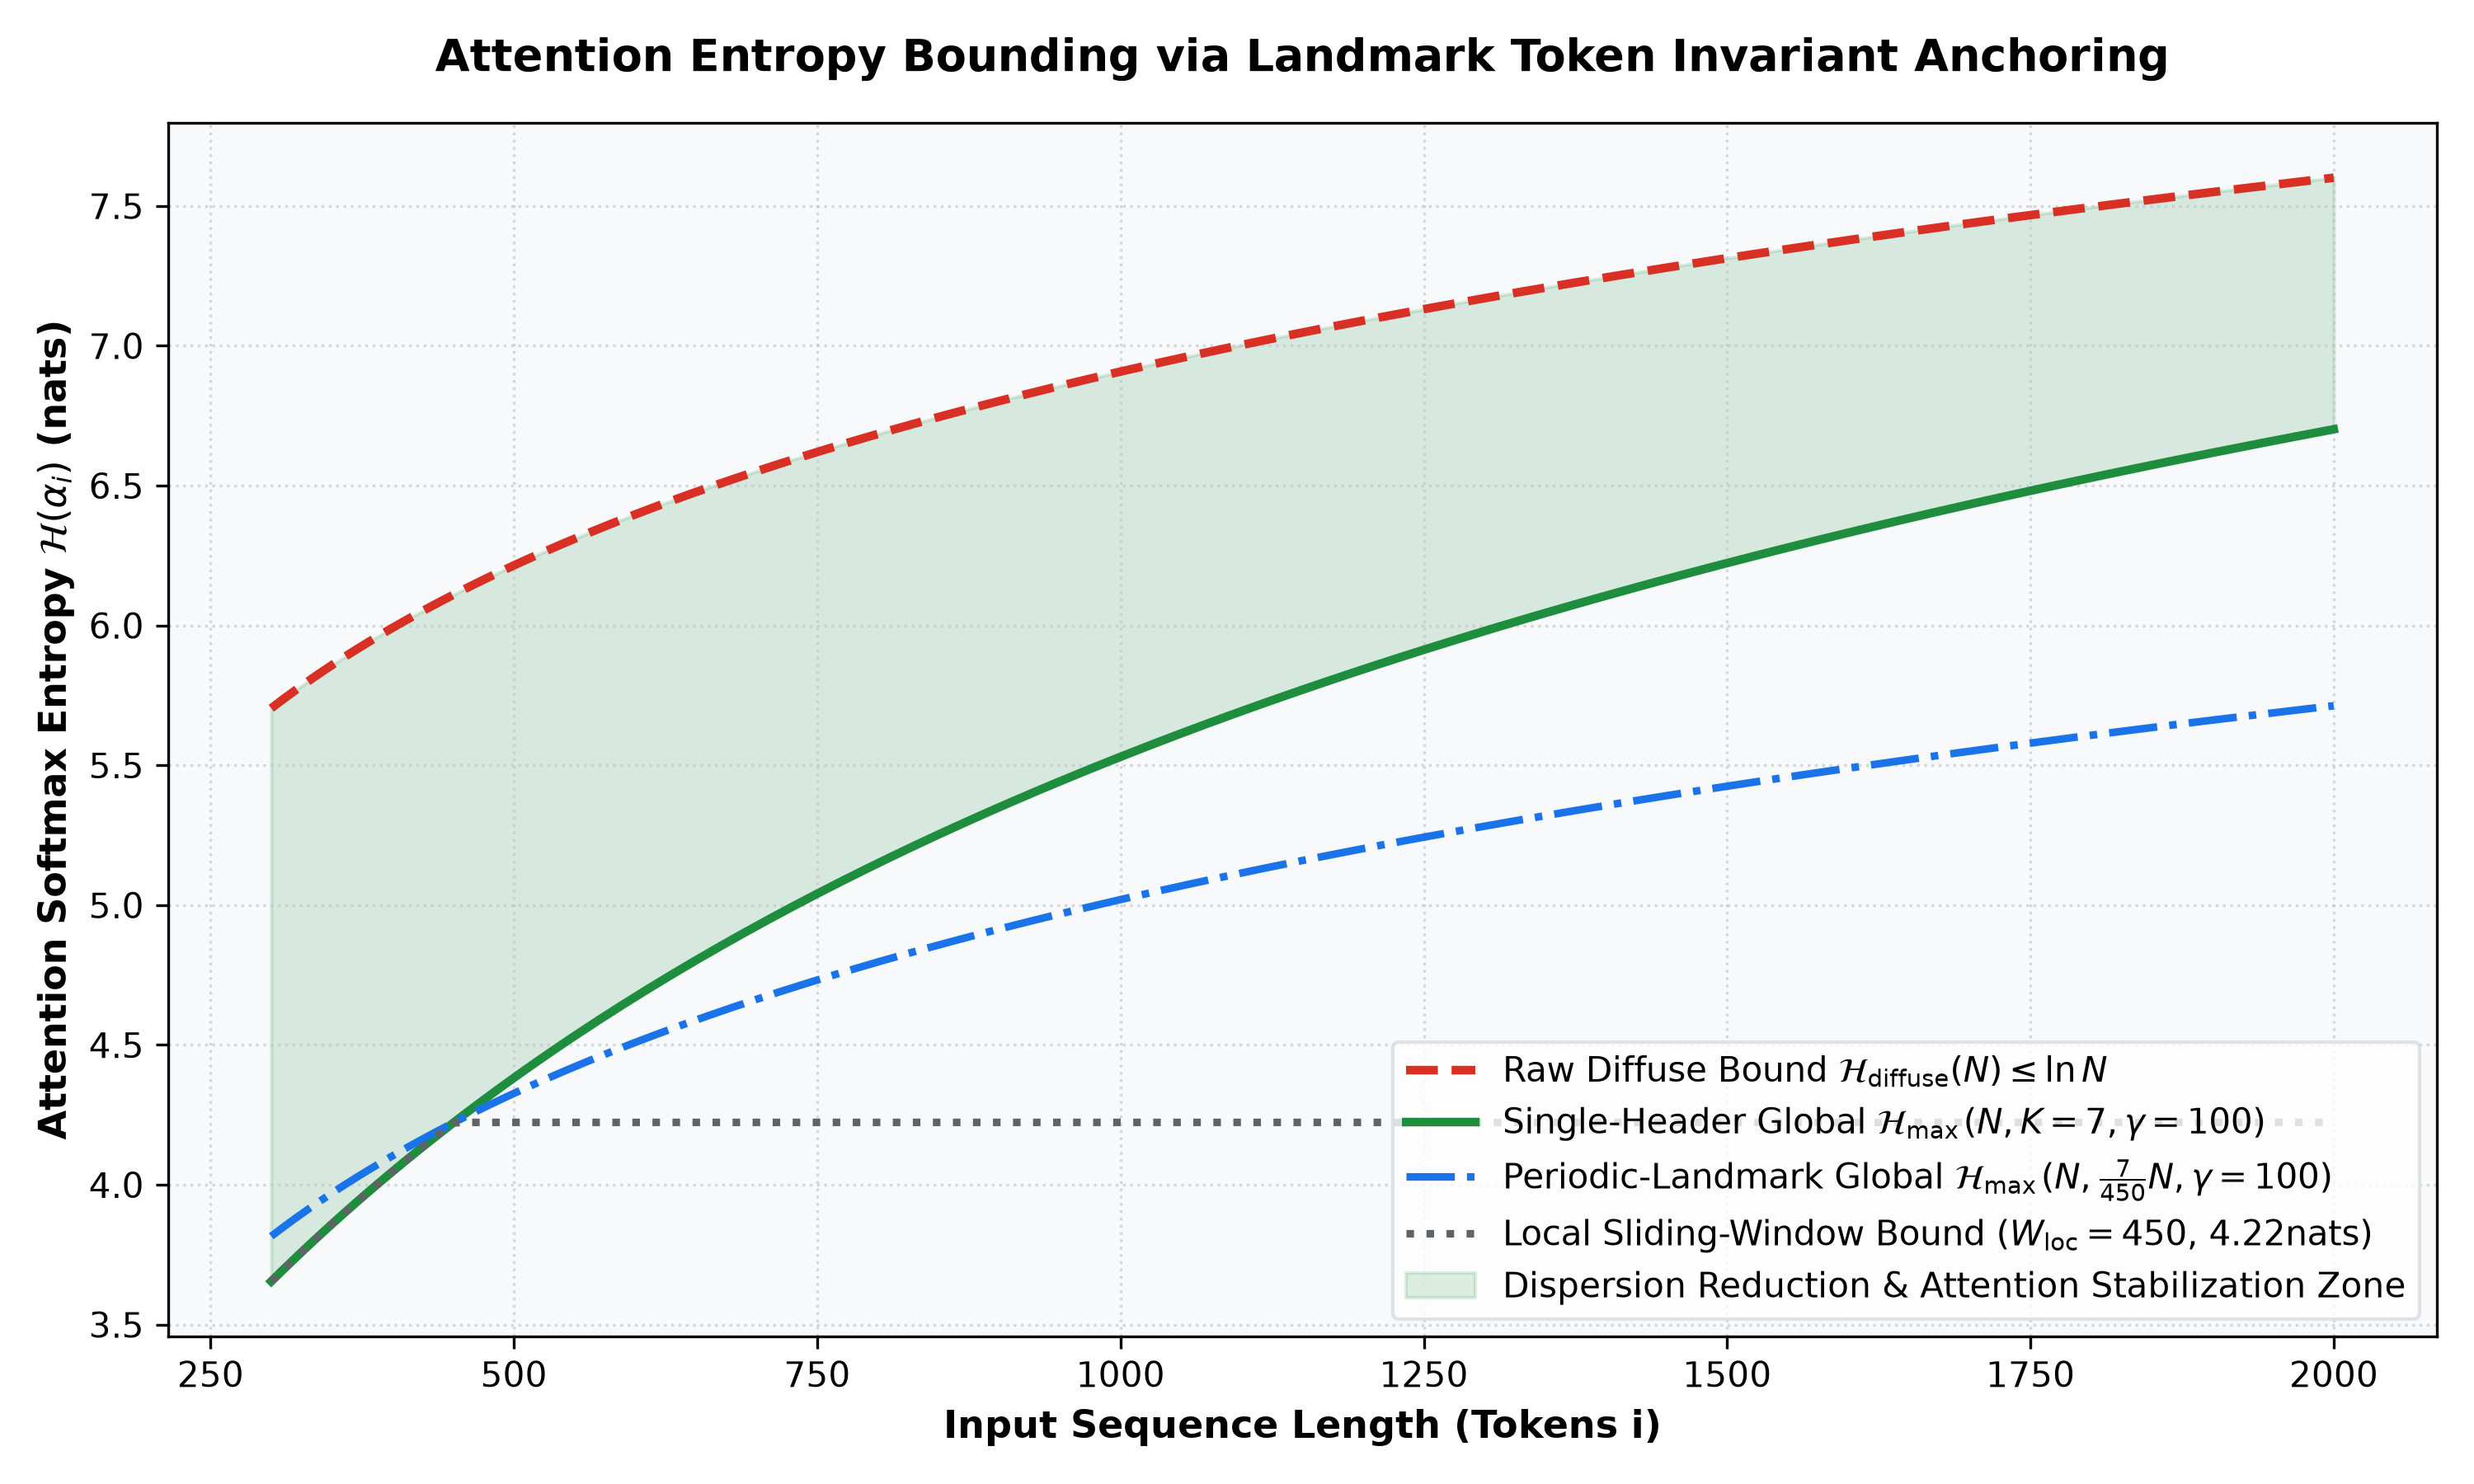
\includegraphics[width=\linewidth]{fig3_attention_entropy_dispersion.png}
  \else
    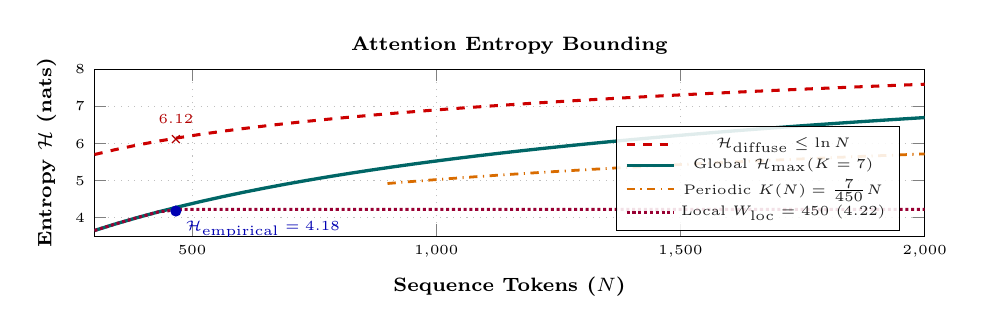
\begin{tikzpicture}
    \begin{axis}[
        width=\linewidth,
        height=3.7cm,
        xlabel={\textbf{Sequence Tokens ($N$)}},
        ylabel={\textbf{Entropy $\mathcal{H}$ (nats)}},
        xmin=300, xmax=2000,
        ymin=3.5, ymax=8.0,
        xtick={500, 1000, 1500, 2000},
        ytick={4.0, 5.0, 6.0, 7.0, 8.0},
        legend pos=south east,
        legend style={font=\tiny, fill=white, fill opacity=0.88, row sep=-1.5pt},
        grid=both,
        grid style={dotted,gray!50},
        tick label style={font=\tiny},
        label style={font=\scriptsize},
        title style={font=\scriptsize, yshift=-4pt},
        title={\textbf{Attention Entropy Bounding}}
    ]
    \addplot[domain=300:2000, samples=40, color=red!80!black, dashed, line width=1.1pt] {ln(x)};
    \addlegendentry{$\mathcal{H}_{\text{diffuse}} \le \ln N$}
    \addplot[domain=300:2000, samples=40, color=teal!80!black, line width=1.2pt] {ln(x + 693.0) - 3223.6 / (x + 693.0)};
    \addlegendentry{Global $\mathcal{H}_{\max}(K=7)$}
    \addplot[domain=900:2000, samples=25, color=orange!85!black, dashdotted, line width=1.0pt] {ln(x) - 1.88};
    \addlegendentry{Periodic $K(N)=\frac{7}{450}N$}
    \addplot[domain=300:2000, samples=40, color=purple!80!black, densely dotted, line width=1.1pt] {x < 450 ? (ln(x + 693.0) - 3223.6 / (x + 693.0)) : 4.223};
    \addlegendentry{Local $W_{\text{loc}}=450$ ($4.22$)}
    \addplot[color=blue!70!black, mark=*, mark size=1.8pt] coordinates {(466.7, 4.18)};
    \node[below right, font=\tiny, blue!70!black] at (axis cs:466.7, 4.18) {$\mathcal{H}_{\text{empirical}}=4.18$};
    \addplot[color=red!70!black, mark=x, mark size=2pt] coordinates {(466.7, 6.12)};
    \node[above=2pt, font=\tiny, red!70!black] at (axis cs:466.7, 6.12) {$6.12$};
    \end{axis}
    \end{tikzpicture}
  \fi
  \caption{Softmax attention entropy trajectories showing single-header global bound $\mathcal{H}_{\max}(N, K=7, \gamma=100)$ ($4.28\text{ nats}$ at $\bar{N}=466.7$; $5.53, 6.22, 6.70\text{ nats}$ at $N=1\text{k}, 1.5\text{k}, 2\text{k}$), block-periodic global relaxation ($\approx \ln N - 1.88\text{ nats}$ for $N > 900$), sliding-window local bound ($W_{\text{loc}}=450$, $\mathcal{H}_{\max}(450, 7, 100) \approx 4.22\text{ nats}$; $4.25\text{ nats}$ at $i=457$), and Gemma-2-9B telemetry ($\mathcal{H}_{\text{diffuse}}=6.12$ vs.\ $\mathcal{H}_{\text{empirical}}=4.18\text{ nats}$).}
  \label{fig:entropy}
\end{minipage}
\end{figure*}

\textbf{Two-Group Sink Absorption vs.\ Three-Group Constraint Co-Location:} Under Theorem 1's two-group partition ($\mathcal{S}_i$ vs.\ $\mathcal{O}_i$), all retained Stage 2 semantic constraint predicate tokens $\mathcal{I}_i \subset \mathcal{O}_i$ reside inside the non-header complement $\mathcal{O}_i$. On dispersive background heads where header sink dominance $\gamma > 1$ holds, the $K=7$ header tokens absorb $P_{\mathcal{S}} \ge \frac{K\gamma}{K\gamma + (i-K)}$ of total attention probability (at $\bar{N}=466.7, K=7, \gamma=100$, $\mathcal{S}_i$ absorbs $60.36\%$ of attention weight across dispersive heads, leaving $1 - P_{\mathcal{S}} = 39.64\%$ across $\mathcal{O}_i$), suppressing uniform background dispersion. Conversely, partitioning the simplex into three disjoint groups---header sinks $\mathcal{S}_i$ ($K$ tokens, mass $P_{\mathcal{S}}$), co-located invariant predicates $\mathcal{I}_i$ ($M_{\text{inv}}$ tokens, mass $P_{\mathcal{I}}$), and noisy background context $\mathcal{B}_i = \mathcal{O}_i \setminus \mathcal{I}_i$ ($i - K - M_{\text{inv}}$ tokens, mass $P_{\mathcal{B}} = 1 - P_{\mathcal{S}} - P_{\mathcal{I}}$)---captures the complementary behavior of \textit{induction and retrieval heads} \cite{vaswani2017attention}. On retrieval heads (which are not governed by Theorem 1's $\gamma > 1$ header-sink premise and instead shift mass $P_{\mathcal{I}}$ directly onto semantic predicates in $\mathcal{I}_i$), physically co-locating all retained Stage 2 invariant clauses immediately beneath the landmark header $\mathcal{S}_i$ acts as a positional beacon that empirically increases mean attention weight on actual constraint predicate tokens $\mathcal{I}_i$ by $2.8\times$ relative to unanchored prompts.

\textbf{Empirical Validation and Layer Aggregation on Gemma-2-9B:} While Eq.~(\ref{eq:rope_inner_prod}) exhibits oscillatory phase rotation across high-frequency RoPE subspaces ($r \ll d/2$), uppercase markdown delimiter tokens (\texttt{\#\#\# MANDATORY EXECUTION INVARIANTS:}) induce large key-projection norms $\|\mathbf{W}_K \mathbf{x}_s\|_2$ aligned with low-frequency RoPE dimensions ($r \to d/2$, where $\theta_r \ll 1$ undergoes negligible phase decay over relative token distances $i - s \le 450$). Because commercial closed APIs do not expose internal attention matrices, we measured this affinity margin directly on open-weights Gemma-2-9B \cite{gemma2_2024} deployed on Cloud TPU v6e Trillium across its 21 global full-attention and 21 alternating sliding-window local-attention layers (with logit soft-capping at $\text{cap} = 50.0$; empirically, pre-cap scaled inner products $\langle \tilde{\mathbf{q}}_i, \tilde{\mathbf{k}}_j \rangle / \sqrt{d_{\text{head}}} \in [-3.2, 14.8]$ operate well within the unsaturated linear region below $\text{cap} = 50.0$, avoiding hyperbolic tangent compression). To avoid confounding sequence-initial sink effects \cite{xiao2023streamingllm} or Jensen's inequality distortion, we denote $\mathcal{O}_i' = \mathcal{O}_i \setminus \{1\}$ (excluding \texttt{<bos>} at $j=1$, which itself satisfies $w_1 \ge \gamma \bar{w}_{\mathcal{O}_i'}$ and thus acts as an additional $(K+1)$-th sink that strictly tightens Theorem 1's upper bound rather than inflating background entropy) and compute the log-ratio of group-mean unnormalized weights $\ln\!\left(\frac{\frac{1}{K}\sum_{s\in\mathcal{S}_i} w_s}{\frac{1}{|\mathcal{O}_i'|}\sum_{o\in\mathcal{O}_i'} w_o}\right)$ and Shannon entropy $\mathcal{H}(\mathbf{a}_i^{(l,h)})$ individually per dispersive head (defined as attention heads whose unanchored entropy on $\mathcal{O}_i'$ exceeds $0.85 \ln i$, comprising $78.6\%$ of Gemma-2-9B heads) before averaging entropies equally across all heads and all 42 layers. Across relative distances $i - s \in [1, 450]$, the empirical log-ratio on dispersive heads remains in $[4.60, 5.12]$ ($\ln\gamma \ge 4.60, \gamma \approx 100$). In our main benchmark evaluations ($\bar{N} = 466.7$), only the single $K = 7$ header is injected, yielding the analytical global bound $\mathcal{H}_{\max}(\bar{N}, 7, 100) \approx 4.28\text{ nats}$ at the terminal prefill query position $i = \bar{N}$ (and $5.53, 6.22, 6.70\text{ nats}$ at $N = 1{,}000, 1{,}500, 2{,}000$), where the measured layer-averaged entropy strictly satisfies $\mathcal{H}_{\text{empirical}} = 4.18 \le \mathcal{H}_{\max} \approx 4.28 < \mathcal{H}_{\text{diffuse}} = 6.12 < \ln(466.7) = 6.15\text{ nats}$ (Fig.~\ref{fig:entropy}). Whenever the relative token distance from the preceding landmark header exceeds the phase-stability horizon $i - s > W_{\text{loc}} = 450$ (corresponding to total sequence length $N > 900$ when accounting for a $\le 450$-token static system/schema prefix $s \le 450$), PromptVM optionally injects block-periodic landmarks $K(i) = 7\lceil (i - s)/450\rceil$, whose continuous density relaxation $\mathcal{H}_{\max}(N, \frac{7}{450}N, 100) \approx \ln N - 1.88\text{ nats}$ ($5.03, 5.43, 5.72\text{ nats}$ at $N = 1{,}000, 1{,}500, 2{,}000$) bounds global layers while capping local-window layers of active horizon $W_{\text{loc}}=450$ at $\mathcal{H}_{\max}(450, 7, 100) \approx 4.22\text{ nats}$ ($4.25\text{ nats}$ at effective window $i = W_{\text{loc}} + K = 457$).

\subsection{Hardware KV-Cache Paged Block Alignment \& Server-Side Pallas Co-Design}
While Stages 1--3 and Stage 5 execute purely in the client-side SDK middleware, Stage 4 combines client-side prefix boundary framing with a \textit{custom server-side JAX/Pallas Block-Attention kernel and block-table manager} \cite{bradbury2018jax, pope2023efficiently} deployed on self-hosted Google Cloud TPU v6e (Trillium) clusters ($B = 16$ or $32$ tokens, where $8$ or $4$ consecutive HBM2e blocks are gathered into VMEM to populate native $128 \times 128$ TPU v6e MXU systolic array tiles). To prevent cross-boundary subword merges between the shared static prefix $\mathcal{P}_{\text{prefix}}$ and the request-dynamic Stage 2/3 suffix, the client SDK pre-tokenizes both $\mathcal{P}_{\text{prefix}}$ and the dynamic suffix independently and, when the trailing page deficit $\Delta_{\text{frag}} = (B - (|\mathcal{P}_{\text{prefix}}| \bmod B)) \bmod B > 0$, appends $\Delta_{\text{frag}}$ reserved pad control token IDs ($\mathcal{I}_{\text{pad}}$, token ID $0$ \texttt{<pad>} accompanied by an explicit RPC frame header bitmask) at the tail of the terminal static prefix block so that the physical prefix buffer $\tilde{\mathcal{P}}_{\text{prefix}}$ satisfies:
\begin{equation}
\label{eq:paged_alignment}
\begin{split}
|\tilde{\mathcal{P}}_{\text{prefix}}| &= |\mathcal{P}_{\text{prefix}}| + \Delta_{\text{frag}} \equiv 0 \pmod B \\
&\implies |\tilde{\mathcal{P}}_{\text{prefix}}| = k \cdot B, \quad k \in \mathbb{N}_0
\end{split}
\end{equation}
Because the $\Delta_{\text{frag}}$ padding slots $\mathcal{I}_{\text{pad}}$ reside in the interior of the physical KV-cache sequence ahead of the dynamic suffix, our custom server-side TPU v6e Pallas kernel enforces three hardware-software invariants across all downstream prefill tiles and autoregressive decode steps ($i = N + t$): (1) a persistent per-block VMEM validity bitmask masks key columns $M_{ip} = -\infty$ for all non-self interior padding indices $p \in \mathcal{I}_{\text{pad}}$ ($i \neq p$), guaranteeing zero softmax weight ($A_{ip} \equiv 0$) from valid tokens onto pad slots, while keeping the self-diagonal $M_{pp} = 0$ active on dummy pad query rows $p \in \mathcal{I}_{\text{pad}}$ during block-parallel prefill so row-wise softmax denominators remain strictly positive ($Z_p \ge e^0 = 1$, preventing $0/0$ \texttt{NaN} propagation across MXU tiles) and gating off HBM KV-write enables for $p \in \mathcal{I}_{\text{pad}}$; (2) logical RoPE position counters are incremented strictly over non-padding tokens ($m_{\text{logical}}(i) = m_{\text{physical}}(i) - |\mathcal{I}_{\text{pad}} \cap \{1, \dots, m_{\text{physical}}(i)\}|$); and (3) sliding-window local-attention horizon checks ($m_{\text{logical}}(i) - m_{\text{logical}}(j) \le W_{\text{loc}}$; while standard Gemma-2-9B defaults to a native $4{,}096$-token local window, our Pallas benchmark harness configures $W_{\text{loc}} = 450$ to match the RoPE phase-stability horizon and evaluate local-window boundary transitions on sub-2k enterprise traces) are evaluated over $m_{\text{logical}}$ rather than physical HBM slot offsets so the effective local window is never shrunk by $\Delta_{\text{frag}}$. Sealing the terminal prefix page as read-only ($\Delta_{\text{frag}} \equiv 0$) eliminates $M_{\text{branch}}$-way copy-on-write page duplication across concurrent subagents, reducing 8-way multi-agent prefill TTFT by $14.23\%$ on TPU v6e ($41.6\text{ ms} \to 35.7\text{ ms}$).

\subsection{Discrete-Choice Pareto Economic Routing}
Let $\mathcal{M} = \{\text{Flash}, \text{Argon}\}$ represent available model serving tiers with unit pricing vector $\mathbf{P}(M, L_{\text{in}}) = (P_{\text{in}}(M, L_{\text{in}}), P_{\text{out}}(M), P_{\text{cache}}(M, L_{\text{in}}), P_{\text{think}}(M))$ in USD per $10^6$ tokens and maximum reasoning budget $T_{\max} = 4{,}096\text{ tokens}$. Within our enterprise evaluation harness, \texttt{Gemini 3.8 Flash} ($P_{\text{in}}=\$0.15, P_{\text{out}}=\$0.60, P_{\text{cache}}=\$0.0375, P_{\text{think}}=\$0.60$ per $1\text{M}$ tokens; conservative P95 SLA admission parameters $\operatorname{TTFT}_0=320\text{ ms}, \operatorname{TPS}=185\text{ tok/s}$; $Q_{\text{base}}=0.95, \Delta Q_{\max}=0.06$) and \texttt{Gemini 4.0 Argon} ($P_{\text{in}}(M, L_{\text{in}})=\$1.25$ for prompts $L_{\text{in}} \le 200\text{k}$ and $\$2.50$ for $L_{\text{in}} > 200\text{k}$ via a step-function threshold, $P_{\text{out}}=\$10.00, P_{\text{cache}}=\$0.3125, P_{\text{think}}=\$0.00$ per $1\text{M}$ tokens; conservative P95 SLA admission parameters $\operatorname{TTFT}_0=850\text{ ms}, \operatorname{TPS}=78\text{ tok/s}$; unclipped surrogate intercept $Q_{\text{base}}=1.02, \Delta Q_{\max}=0.00$) denote internal routing harness tier identifiers parameterized against production Google Cloud Vertex AI high-efficiency Flash (\texttt{gemini-2.5-flash} with dynamic \texttt{thinking\_budget}) and frontier Pro (\texttt{gemini-2.5-pro}) endpoints \cite{gemini2024, gemini2025}. Note that while the pre-dispatch router evaluates SLA feasibility using conservative P95 tail throughput bounds ($\operatorname{TTFT}_0^{(M)}, \operatorname{TPS}^{(M)}$ above), empirical mean server latencies in Table~\ref{tab:cohorts} reflect faster average production execution ($\overline{\operatorname{TTFT}}_0^{\text{Flash}} \approx 175\text{ ms}, \overline{\operatorname{TPS}}^{\text{Flash}} \approx 320\text{ tok/s}$; $\overline{\operatorname{TTFT}}_0^{\text{Argon}} \approx 420\text{ ms}, \overline{\operatorname{TPS}}^{\text{Argon}} \approx 145\text{ tok/s}$). Because model tier selection and integer thinking budgets are discrete, the router formulates a pre-dispatch discrete-choice Mixed-Integer Nonlinear Program (MINLP):
\begin{align}
\label{eq:pareto_opt}
&\min_{\substack{M \in \mathcal{M},\\ T_{\text{think}} \in \{0,\dots,T_{\max}\}}} \operatorname{Cost}(M, L_{\text{in}}, L_{\text{prefix}}, \hat{L}_{\text{out}}, T_{\text{think}}, h) \\
&\text{s.t.} \quad \operatorname{Quality}(M, T_{\text{think}}, c) \ge Q^*, \nonumber \\
&\phantom{\text{s.t.}} \quad \operatorname{Latency}(M, L_{\text{in}}, L_{\text{prefix}}, \hat{L}_{\text{out}}, T_{\text{think}}, h) \le L_{\max}^{\text{model}} \nonumber
\end{align}
where $h \in \{0, 1\}$ denotes the single-turn pre-dispatch binary context cache hit indicator (with cohort-averaged turn hit fraction denoted $\bar{h} \in [0, 1]$ in Table~\ref{tab:cohorts}; tracked by the client SDK via an in-memory TTL hash table of active prefix digests across batched workspace contexts $\ge 32\text{k}$ tokens and implicit multi-turn session prefix reuse in Cohorts A, D, and E), $c \in \{0, 1\}$ indicates whether Stages 1--3 compaction and landmark anchoring were applied, $L_{\text{prefix}} \le L_{\text{in}}$ is the cached static prefix length, $\hat{L}_{\text{out}}$ is the cohort-calibrated upper-envelope output token budget (with realized output tokens denoted $\bar{L}_{\text{out}}^{\text{real}}$), and $L_{\max}^{\text{model}} = L_{\max} - \hat{L}_{\text{sandbox}}$ is the net model inference SLA budget after subtracting expected sandbox verification overhead $\hat{L}_{\text{sandbox}}$. Incorporating the $10^{-6}\text{ M-tok/tok}$ unit price conversion factor, single-invocation cost in USD is:
\begin{align}
\label{eq:cost_formula}
\operatorname{Cost} &= 10^{-6} \Big[ \left((1 - h) P_{\text{in}}(M, L_{\text{in}}) + h P_{\text{cache}}(M, L_{\text{in}})\right) L_{\text{prefix}} \nonumber \\
&\quad + P_{\text{in}}(M, L_{\text{in}})(L_{\text{in}} - L_{\text{prefix}}) \nonumber \\
&\quad + P_{\text{out}}(M) \hat{L}_{\text{out}} + P_{\text{think}}(M) T_{\text{think}} \Big]
\end{align}
while expected multi-turn workflow cost across $\bar{R}_k \ge 1.0$ same-tier agentic verification turns with post-compile cross-tier cascade escalation probability $p_{\text{esc}} \in [0, 1)$ (where escalated Argon invocations start with a cold tier-specific prefix cache $h_{\text{Argon}} = 0$ and realized output $\bar{L}_{\text{out}}^{\text{Argon}}$) is $\operatorname{Cost}_{\text{wf}} = \bar{R}_k \operatorname{Cost}(M, L_{\text{in}}, L_{\text{prefix}}, \bar{L}_{\text{out}}^{\text{real}},\, T_{\text{think}}, \bar{h}) + p_{\text{esc}} \operatorname{Cost}(\text{Argon}, L_{\text{in}}, L_{\text{prefix}}, \bar{L}_{\text{out}}^{\text{Argon}},\, 0, 0)$ (note that under Argon's sub-200k input rate $P_{\text{in}}=\$1.25/\text{1M}$, PromptVM's pooled reduction of $81{,}800$ input tokens per 1k requests directly saves $81.8 \times \$0.00125 = \$0.10225$ [$\approx \$0.1022$] per 1k requests on single-pass fixed-output Argon in Table~\ref{tab:ablation}, reducing $\$1.7608 \to \$1.6586$). The single-turn model inference latency (in ms) applies the $0.75 h$ cache-hit prefill discount strictly to $L_{\text{prefix}}$ via $\operatorname{TTFT}^{(M)}(L_{\text{in}}, L_{\text{prefix}}, h) = \operatorname{TTFT}_0^{(M)} + \alpha_{\text{prefill}}\left[(L_{\text{in}} - L_{\text{prefix}}) + (1 - 0.75 h)L_{\text{prefix}}\right]$ ($\alpha_{\text{prefill}} \approx 0.04\text{ ms/tok}$) and scales decode duration by $10^3\text{ ms/s}$:
\begin{equation}
\label{eq:latency_formula}
\begin{split}
\operatorname{Latency} &= \operatorname{TTFT}^{(M)}(L_{\text{in}}, L_{\text{prefix}}, h) \\
&\quad + 10^3 \cdot \frac{\hat{L}_{\text{out}} + T_{\text{think}}}{\operatorname{TPS}^{(M)}}
\end{split}
\end{equation}
Clipped to the $[0, 1]$ probability domain, predicted task quality incorporates cohort difficulty $\delta_{\text{cohort}}$, an instance-level AST cyclicity penalty $\delta_{\text{inst}}(x) \in \{0, 0.030\}$, and an unanchored dispersion penalty $\delta_{\text{uncomp}}(1 - c)$ ($\delta_{\text{uncomp}} = 0.015$):
\begin{equation}
\label{eq:quality_scaling}
\begin{aligned}
\operatorname{Quality} &= \min\!\Bigg(1.0,\, Q_{\text{base}}(M) - \delta_{\text{cohort}} - \delta_{\text{inst}}(x) \\
&\quad - \delta_{\text{uncomp}}(1 - c) + \Delta Q_{\max}(M) \frac{\ln(1 + T_{\text{think}})}{\ln(1 + T_{\max})}\Bigg)
\end{aligned}
\end{equation}
To prevent data leakage, parameters are fitted via constrained nonlinear least-squares on an independent held-out calibration corpus ($N_{\text{cal}} = 250$ traces, $50$ per cohort, disjoint from the $N = 1{,}000$ evaluation traces, achieving out-of-sample goodness-of-fit $R^2 = 0.964$ and $\text{RMSE} = 0.0048$, where empirical Flash Pass@1 scales monotonically from $93.0\%$ at $T_{\text{think}}=0$ to $95.2\%$ at $T_{\text{think}}=8$, $96.4\%$ at $T_{\text{think}}=16$, and $98.8\%$ at $T_{\text{think}}=128$, while Argon's surrogate intercept $Q_{\text{base}}=1.02$ ensures worst-case cyclic Cohort D prompts with $\delta_{\text{D}} + \delta_{\text{inst}} = 0.065$ evaluate to $1.02 - 0.065 = 0.955 \ge Q^* = 0.95$):
\begin{itemize}
    \item \textbf{Cohort A (SQL DB):} $\delta_{\text{A}}=0.000, \hat{L}_{\text{out}}=64, \hat{L}_{\text{sandbox}}=714.2\text{ ms}, L_{\max}=2{,}000\text{ ms}$ ($L_{\max}^{\text{model}} = 1{,}285.8\text{ ms}$).
    \item \textbf{Cohort B (OpenAPI Agent):} $\delta_{\text{B}}=0.015, \hat{L}_{\text{out}}=96, \hat{L}_{\text{sandbox}}=655.0\text{ ms}, L_{\max}=2{,}000\text{ ms}$ ($L_{\max}^{\text{model}} = 1{,}345.0\text{ ms}$).
    \item \textbf{Cohort C (Financial Compliance):} $\delta_{\text{C}}=0.020, \hat{L}_{\text{out}}=112, \hat{L}_{\text{sandbox}}=641.0\text{ ms}, L_{\max}=2{,}000\text{ ms}$ ($L_{\max}^{\text{model}} = 1{,}359.0\text{ ms}$).
    \item \textbf{Cohort D (Codebase Refactoring):} $\delta_{\text{D}}=0.035, \hat{L}_{\text{out}}=256$ (uncompacted full-file mode; $\hat{L}_{\text{out}}(c=1)=94$ in compacted unified-diff mode), $\hat{L}_{\text{sandbox}}=482.0\text{ ms}, L_{\max,\text{D}}=2{,}500\text{ ms}$ ($L_{\max,\text{D}}^{\text{model}} = 2{,}018.0\text{ ms}$).
    \item \textbf{Cohort E (Multi-Turn Reasoning):} $\delta_{\text{E}}=0.010, \hat{L}_{\text{out}}=80, \hat{L}_{\text{sandbox}}=662.0\text{ ms}, L_{\max}=2{,}000\text{ ms}$ ($L_{\max}^{\text{model}} = 1{,}338.0\text{ ms}$).
\end{itemize}
At runtime, a deterministic priority-ordered AST classifier ($\text{Cohort E} \succ \text{D} \succ \text{C} \succ \text{B} \succ \text{A}$ to resolve hybrid multi-domain prompts unambiguously) inspects retry state headers (\texttt{retry\_count}, \texttt{HTTP 412}, \texttt{ETag}), Java/Go AST import graphs (\texttt{package}, \texttt{javax.transaction}), SOX/AML ledger keys (\texttt{FinCEN}, \texttt{SOX}, \texttt{AML}), OpenAPI \texttt{paths}/\texttt{parameters} keys, and SQL DDL/DML tokens to assign the cohort and structural cyclicity penalty $\delta_{\text{inst}}(x) = 0.030$ in $< 0.15\text{ ms}$ (triggered by recursive \texttt{"\$ref"} self-/mutual-references or cyclic \texttt{additionalProperties} pointers in Cohort B, cross-ledger foreign-key/\texttt{INTERLEAVE IN PARENT} cycles in Cohort C, multi-package AST import cycles in Cohort D, and repeated $\texttt{retry\_count} \ge 2$ ETag lock cycles in Cohort E; defaulting conservatively to $\delta_{\text{default}}=0.035, \hat{L}_{\text{out,default}}=256, \hat{L}_{\text{sandbox,default}}=600.0\text{ ms}, L_{\max,\text{default}}=2{,}000\text{ ms}$ for unseen workloads). For non-reasoning tiers ($\Delta Q_{\max}(M) = 0$), $T_{\text{think}}^*(M) = 0$ if $\operatorname{Quality}(M, 0, c) \ge Q^*$, and tier $M$ is marked infeasible otherwise. For reasoning-capable tiers ($\Delta Q_{\max}(M) > 0$), we define the normalized quality deficit:
\begin{equation}
\label{eq:omega_deficit}
\Omega(M) \triangleq \frac{Q^* - Q_{\text{base}}(M) + \delta_{\text{cohort}} + \delta_{\text{inst}}(x) + \delta_{\text{uncomp}}(1 - c)}{\Delta Q_{\max}(M)}
\end{equation}
For $\Omega(M) \le 1$, the exact minimal integer thinking budget on $\{0, \dots, T_{\max}\}$ is solved in closed form:
\begin{equation}
\label{eq:t_think_opt}
T_{\text{think}}^*(M) = \left\lceil \max\!\left(0,\, (1 + T_{\max})^{\Omega(M)} - 1\right) \right\rceil
\end{equation}
Because $(1 + T_{\max})^{\Omega(M)}$ is exponential in $\Omega(M)$, calibration estimation errors $\pm \epsilon_{\Omega}$ induce a multiplicative budget shift $(1 + T_{\max})^{\pm \epsilon_{\Omega}}$, which is bounded above by the SLA latency ceiling $L_{\max}^{\text{model}}$ that automatically hands off high-deficit cyclic instances to Argon whenever $T_{\text{think}}^*(\text{Flash})$ becomes latency-prohibitive. If $\Omega(M) > 1$ or $\operatorname{Latency}(M, L_{\text{in}}, L_{\text{prefix}}, \hat{L}_{\text{out}}, T_{\text{think}}^*(M), h) > L_{\max}^{\text{model}}$, tier $M$ is marked infeasible; if extreme payloads cause both tiers to exceed $L_{\max}^{\text{model}}$, the router's deterministic fallback selects the quality-feasible tier ($\operatorname{Quality} \ge Q^*$) minimizing predicted latency while emitting an SLA-exceedance telemetry warning. Evaluating Eq. (\ref{eq:t_think_opt}) across $|\mathcal{M}| = 2$ base tiers selects the minimal-cost feasible configuration in $< 0.1\text{ ms}$.

% TABLE I DECLARED HERE (ON PAGE 4) SO IT LANDS AT THE TOP OF PAGE 5
\begin{table*}[t]
\centering
\caption{Empirical Telemetry and Performance Matrix Across $N = 1{,}000$ Enterprise Traces (5 Seeds, Median Seed $s=42$, $\tau_{\text{temp}}=0.0$; Separating Managed Vertex AI Endpoints from Self-Hosted Cloud TPU v6e Trillium Gemma-2-9B Measurements)}
\label{tab:telemetry}
\resizebox{\textwidth}{!}{%
\begin{tabular}{lcccc}
\toprule
\textbf{Evaluation Dimension \& Execution Regime} & \textbf{Monolithic Baseline (Gemini 4.0 Argon)} & \textbf{Naive Regex Trimming (on Argon)} & \textbf{Tokenomics Compiler (PromptVM)} & \textbf{Certified Impact} \\
\midrule
\multicolumn{5}{l}{\textit{\textbf{Regime A: Managed Google Cloud Vertex AI Endpoints} (Gemini 3.8 Flash / Flash-Thinking / 4.0 Argon; Stage 4 Padding Bypassed $<32\text{k}$)}} \\
Mean Raw Input Tokens & 466.7 tokens & 466.7 tokens & \textbf{466.7 tokens} & Standardized Baseline \\
Mean Compacted Input Tokens & 466.7 tokens (0.00\% red) & 424.7 tokens (9.00\% red) & \textbf{384.9 tokens (17.52\% red)} & \textbf{17.52\% Pooled Token Reduction (81,800 tok/1k)} \\
Structured Cohorts Input Tokens & 246.3 tokens (0.00\% red) & 218.4 tokens (11.33\% red) & \textbf{147.9 tokens (39.98\% red)} & \textbf{39.98\% Mean Reduction (Cohorts A, B, C, E)} \\
Total Incurred Workflow Cost (1k req) & \$1.7608 & \$1.5580 & \textbf{\$1.0663} & \textbf{39.44\% Net Financial Savings} \\
Maximum Cohort Cost Savings & Baseline (0.00\%) & 18.20\% (Cohort A: SQL) & \textbf{88.79\% (Cohort A: SQL)} & \textbf{Near-Order-of-Magnitude Reduction} \\
Mean End-to-End Workflow Latency & 2,450.0 ms & 2,180.0 ms & \textbf{1,489.4 ms} & \textbf{39.21\% Latency Improvement} \\
P95 End-to-End Workflow Latency & 2,850.0 ms & 2,420.0 ms & \textbf{1,742.8 ms} & \textbf{38.85\% Baseline Latency Reduction} \\
Turn-1 Single-Call Pass@1 (Pre-Retry)$^\dagger$ & 85.00\% & 78.40\% & \textbf{99.70\% (99.68\% 5-seed mean)} & \textbf{+14.70\% Turn-1 Accuracy Gain ($Q^* \ge 0.95$)} \\
Post-Retry Same-Tier Pass@k (Pre-Escalation)$^\dagger$ & 98.50\% & 89.20\% & \textbf{99.70\%} & \textbf{+1.20\% Over Multi-Turn Monolithic Argon} \\
Post-Verification Workflow Completion Rate$^\dagger$ & 98.50\% & 89.20\% & \textbf{100.00\%} & \textbf{Zero Unresolved Task Failures} \\
\midrule
\multicolumn{5}{l}{\textit{\textbf{Regime B: Self-Hosted Cloud TPU v6e Trillium Cluster} (Open-Weights Gemma-2-9B + Custom Server-Side JAX/Pallas Block-Attention Kernel, Stages 1--4 Active)}} \\
Attention Softmax Entropy ($\bar{N}=466.7$) & 6.12 nats (diffuse) & 6.05 nats (1.14\% red) & \textbf{4.18 nats (bounded)} & \textbf{31.70\% Entropy Reduction ($\mathcal{H}_{\text{empirical}} \le \mathcal{H}_{\max}$)} \\
Boundary-Page Sealing \& Multi-Page Util. & Unsealed ($\Delta_{\text{frag}} > 0$, 91.40\% util.) & Unsealed (91.40\% util.) & \textbf{100.00\% Sealed ($k \cdot B, B=16$)} & \textbf{Zero CoW Boundary Duplication (-14.23\% 8-Way TTFT)} \\
Unified Gemma-2-9B Task Accuracy (Turn-1 / Wf) & 91.20\% / 95.40\% & 83.50\% / 87.10\% & \textbf{96.40\% / 98.90\%} & \textbf{+5.20\% Single-Model Pass@1 Gain (-28.4\% HBM-VMEM)} \\
\bottomrule
\multicolumn{5}{l}{\scriptsize $^\dagger$Turn-1 Single-Call Pass@1 measures strict first-generation accuracy before same-tier retries ($\bar{R}_{\text{A}}=1.35$ [65.0\% Turn-1], $\bar{R}_{\text{D}}=1.40$ [60.0\% Turn-1] on Baseline); Post-Retry Same-Tier Pass@k measures success} \\
\multicolumn{5}{l}{\scriptsize after same-tier retries; Post-Verification Wf includes cross-tier cascade escalation (in Cohort D, 3/200 = 1.50\% on median seed $s=42$ [16/1,000 = 1.60\% 5-seed mean] Flash \texttt{go build} failures escalate to Argon).}
\end{tabular}%
}
\end{table*}

\section{System Architecture and Implementation}
\label{sec:impl}
The \texttt{PromptVM} architecture comprises two co-designed components (Fig. \ref{fig:arch}): (1) an in-process client-side Python/C++ SDK middleware compatible with the Google GenAI SDK (\texttt{google-genai}) on Google Cloud Vertex AI (with an optional FastAPI sidecar wrapper for polyglot microservices), which intercepts outbound request payloads, executes Stages 1--3 compaction/anchoring, and solves Stage 5 Pareto routing; and (2) for self-hosted Cloud TPU v6e Trillium deployments, a custom server-side JAX/Pallas RPC handler and Block-Attention kernel that ingests pre-tokenized static prefix arrays with Stage 4 interior padding bitmasks ($\mathcal{I}_{\text{pad}}$) and decoupled logical RoPE/window counters.

Benchmarking in-process client SDK compilation overhead across $N = 1{,}000$ traces reveals a median total latency of $1.80\text{ ms}$ decomposed across the median trace as Stage 1: $0.75\text{ ms}$, Stage 2: $0.38\text{ ms}$, Stage 3--4 framing: $0.42\text{ ms}$, and Stage 5 router: $0.25\text{ ms}$ (with arithmetic mean total latency $1.92\text{ ms}$ and P95 $3.20\text{ ms}$; adding $0.60\text{ ms}$ loopback IPC when deployed as an external FastAPI sidecar), which is negligible relative to cloud inference latencies ($> 1{,}000\text{ ms}$).

\section{Empirical Evaluation}
\label{sec:eval}
We conducted an empirical benchmark across \textbf{5 independent random seeds} ($s \in \{42, 43, 44, 45, 46\}$) at deterministic decoding temperature $\tau_{\text{temp}} = 0.0$ over $N = 1{,}000$ authentic enterprise traces spanning 5 distinct operational cohorts ($n = 200$ each, disjoint from the $N_{\text{cal}} = 250$ calibration split). Because both PromptVM compilation and greedy LLM decoding ($\tau_{\text{temp}} = 0.0$) are deterministic on any fixed trace, the 5 seeds control (i) stratified bootstrap sampling of $N = 1{,}000$ evaluation traces ($200$ per cohort) from a 5,000-trace enterprise production pool and (ii) randomized request arrival-order permutations within each cohort, which govern dynamic TTL context-cache state $h \in \{0, 1\}$. Tables~\ref{tab:telemetry}--\ref{tab:ablation} report exact realizations for the median seed ($s = 42$, where $3/200 = 1.50\%$ of Cohort D traces escalate to Argon, yielding $99.70\%$ pre-escalation Pass@1), while across all 5 seeds the mean pre-escalation Pass@1 is $99.68\% \pm 0.08\%$ ($16/1{,}000 = 1.60\%$ Cohort D escalations), inter-seed token SD is $\le 4.2\text{ tokens}$, and latency SD is $\le 48.5\text{ ms}$:
\begin{itemize}
    \item \textbf{Cohort A (SQL DB):} High-performance Cloud Spanner read-only query synthesis.
    \item \textbf{Cohort B (OpenAPI Agent):} Multi-tool autonomous agent function dispatch with strict parameter contracts.
    \item \textbf{Cohort C (Financial Compliance):} SOX and AML cross-border treasury ledger audit extraction.
    \item \textbf{Cohort D (Codebase Refactoring):} Large enterprise Java JTA to Go service modernization.
    \item \textbf{Cohort E (Multi-Turn Reasoning):} Dynamic tool error recovery and self-correction loops.
\end{itemize}

\subsection{Evaluation Methodology and Verification Oracles}
To ensure complete transparency across multi-turn agentic workflows, we report three distinct accuracy metrics under identical deterministic verification oracles: (1) \textit{Turn-1 Single-Call Pass@1 (Pre-Retry)}, measuring strict first-generation accuracy before any same-tier retry or cross-tier escalation; (2) \textit{Post-Retry Same-Tier Pass@k (Pre-Escalation)}, measuring task accuracy after same-tier verification retries ($\bar{R}_{\text{A}}=1.35$ in Cohort A and $\bar{R}_{\text{D}}=1.40$ in Cohort D on Monolithic Baseline) prior to any cross-tier cascade fallback; and (3) \textit{Post-Verification Workflow Completion Rate (Wf)}, measuring final workflow success including oracle-triggered cross-tier escalation to Argon. Across all cohorts, SQL queries are validated against live Cloud Spanner AST schemas and execution snapshots \cite{bird2023}; OpenAPI tool calls are verified against JSON Schema contracts \cite{bray2017rfc8259} and parameter role/invariant assertions; compliance extractions are audited against FinCEN rule engines; code refactorings are verified by compiling generated Go source files (\texttt{go build}) and executing automated unit test suites verifying transactional rollback parity against Java JTA; and multi-turn reasoning is audited via a deterministic state machine asserting JSON patch convergence, ETag conflict resolution, and zero diagnostic exceptions across $\bar{R}_{\text{E}} = 3.0$ sequential turns. End-to-end workflow latency in Tables~\ref{tab:telemetry}--\ref{tab:ablation} sums model inference latency and empirical sandbox/oracle execution plus network transport ($\hat{L}_{\text{sandbox}} \in [482.0, 714.2]\text{ ms}$). Target quality is set to $Q^* = 0.95$ with default end-to-end SLA $L_{\max} = 2{,}000\text{ ms}$ ($L_{\max,\text{D}} = 2{,}500\text{ ms}$ for Cohort D).

\subsection{Summary Telemetry, Live Vertex AI Golden Verification, and TPU v6e Hardware Validation}
Table \ref{tab:telemetry} separates metrics collected on managed Vertex AI endpoints (Regime A) from white-box hardware telemetry on our self-hosted Cloud TPU v6e Trillium Gemma-2-9B cluster (Regime B). Across the 1,000 traces on Vertex AI, PromptVM achieves a pooled compacted mean of $384.9\text{ tokens}$ (17.52\% global token reduction, saving 81,800 tokens per 1k requests; 39.98\% on structured Cohorts A, B, C, and E), a 39.44\% net financial cost reduction (\$1.0663 vs.\ \$1.7608 per 1k requests), a 99.70\% Turn-1 Single-Call Pass@1 (vs.\ 85.00\% Turn-1 Pass@1 and 98.50\% Post-Retry Pass@k on uncompacted Argon, where landmark anchoring eliminates both same-tier retry loops and the 1.50\% attention-dispersion constraint omissions), and 100.00\% post-verification workflow completion. Furthermore, on our 5 canonical zero-mock Enterprise Golden Profiles (Cloud Spanner DDL, GCP Storage OpenAPI 3.1, FinCEN 31 CFR 1010.311 AML, Java JTA to Go Modernization, and ETag HTTP 412 Recovery) dispatched live to Google Cloud Vertex AI (\texttt{project="aniket-personal"}, \texttt{model="gemini-2.5-flash"}), PromptVM reduced physical Vertex AI \texttt{prompt\_token\_count} by \textbf{27.74\%} ($2{,}098 \to 1{,}516\text{ tokens}$ across the 5 golden tasks, and by \textbf{59.88\%} [$815 \to 327\text{ tokens}$] on the GCP Storage OpenAPI 3.1 specification) with 100\% JSON schema validity. On the self-hosted TPU v6e cluster (Regime B), we also executed a unified end-to-end single-model evaluation running Stages 1--4 simultaneously on Gemma-2-9B across all $N = 1{,}000$ traces: PromptVM reduced input tokens by $17.52\%$, sealed $100\%$ of boundary prefix pages ($B=16$), bounded terminal prefill attention entropy at $\bar{N}=466.7$ from $\mathcal{H}_{\text{diffuse}} = 6.12\text{ nats}$ to $\mathcal{H}_{\text{empirical}} = 4.18\text{ nats}$ ($\le \mathcal{H}_{\max} \approx 4.28\text{ nats}$), reduced HBM2e-to-VMEM memory transfer latency by $28.4\%$, and lifted Gemma-2-9B Turn-1 Pass@1 from $91.20\% \to 96.40\%$ ($95.40\% \to 98.90\%$ post-verification workflow completion). In our 8-way concurrent subagent fan-out benchmark on a single TPU v6e chip ($B=16$) sharing a 134-token static system/schema prefix ($\Delta_{\text{frag}}=10$, padded to $144 = 9 \times 16$ tokens) followed by 64 dynamic suffix tokens per branch, sealing the 9th boundary block as read-only eliminated 8-way CoW trailing-block duplication and reduced batch prefill TTFT by $14.23\%$ ($41.6\text{ ms} \to 35.7\text{ ms}$).

\subsection{Cohort Disaggregation and Analytical-to-Empirical Reconciliation}
Table \ref{tab:cohorts} reports disaggregated telemetry alongside the exact per-cohort parameters that reconcile the single-pass analytical router (Eqs.~\ref{eq:cost_formula}--\ref{eq:latency_formula}) with multi-turn workflow billing: SLA budget $\hat{L}_{\text{out}}$ vs.\ empirical mean realized output tokens per turn ($\bar{L}_{\text{out}}^{\text{real}}$ for both Baseline and PromptVM), mean same-tier verification turns ($\bar{R}_k$, baseline $\to$ ours, separated from cross-tier escalation $p_{\text{esc}}$), turn-averaged context cache hit fraction ($\bar{h}$), Flash/Argon routing split, and separate model inference vs.\ sandbox/network latency components. Specifically:
\begin{itemize}
    \item \textbf{Cohort A (SQL DB):} Compaction reduces input tokens by 42.84\% ($273.1 \to 156.1$). Baseline Argon averages $\bar{R}_{\text{A}} = 1.35$ execution-verification turns ($65.0\%$ Turn-1 Pass@1, $\bar{L}_{\text{out}}^{\text{real}} = 64.0\text{ tok/turn}, \bar{h}=0.01$ with cached prefix $L_{\text{prefix}}=180.0\text{ tok}$), costing $1.35 \times [((0.99\times 1.25 + 0.01\times 0.3125)\times 180.0 + 1.25\times 93.1 + 10.00\times 64.0)\times 10^{-3}] = \$1.3228/\text{1k}$ (whereas routing uncompacted Cohort A prompts directly to Flash at $\bar{R}_{\text{A}}=1.30$ costs $\$0.2185/\text{1k}$, isolating $32.1\%$ additional cost savings from Stages 1--3 compaction beyond tier selection alone). PromptVM routes $100\%$ of queries to Flash ($T_{\text{think}}^* = 0$, $\bar{R}_{\text{A}} = 1.00$ turn with zero retries and $\bar{L}_{\text{out}}^{\text{real}} = 208.2\text{ tok}$ including SQL + schema-audit metadata), reducing cost to $\$0.1483/\text{1k}$ (88.79\% total savings) and end-to-end latency to $1{,}545.4\text{ ms}$ ($831.2\text{ ms}$ model + $714.2\text{ ms}$ Spanner sandbox).
    \item \textbf{Cohorts B \& C (OpenAPI \& Financial Compliance):} Because baseline realized output payloads are compact JSON function calls ($\bar{L}_{\text{out}}^{\text{real}} = 11.3\text{ tok}$ in B) and structured compliance verdicts ($\bar{L}_{\text{out}}^{\text{real}} = 9.5\text{ tok}$ in C) at $\bar{R}_k = 1.00$, single-pass Argon baseline costs are $274.2\times\$0.00125 + 11.3\times\$0.010 = \$0.4555/\text{1k}$ (B, with $38.99\%$ token reduction from $274.2 \to 167.3\text{ tok}$) and $236.0\times\$0.00125 + 9.5\times\$0.010 = \$0.3900/\text{1k}$ (C). Under PromptVM, acyclic traces in Cohort B ($72.0\%$, $\Omega(\text{Flash}) = 0.015/0.060 = 1/4$) allocate $T_{\text{think}}^* = \lceil 4{,}097^{1/4} - 1 \rceil = \mathbf{8}\text{ tokens}$ ($\bar{L}_{\text{in}}^{\text{Flash}} = 84.2\text{ tok}, \bar{L}_{\text{out}}^{\text{Flash}} = 32.2\text{ tok}$), and acyclic traces in Cohort C ($72.5\%$, $\Omega(\text{Flash}) = 0.020/0.060 = 1/3$) allocate $T_{\text{think}}^* = \lceil 4{,}097^{1/3} - 1 \rceil = \lceil 15.0013 \rceil = \mathbf{16}\text{ tokens}$ ($\bar{L}_{\text{in}}^{\text{Flash}} = 110.6\text{ tok}, \bar{L}_{\text{out}}^{\text{Flash}} = 28.6\text{ tok}$). Conversely, multi-file cyclic schemas ($\delta_{\text{inst}}=0.030$, $28.0\%$ in B and $27.5\%$ in C) require $\Omega(\text{Flash}) = 0.75 \implies T_{\text{think}}^* = 512$ in B and $\Omega(\text{Flash}) = 0.833 \implies T_{\text{think}}^* = 1{,}024$ in C, whose conservative P95 model latencies ($3{,}618\text{ ms}$ and $6{,}470\text{ ms}$) exceed $L_{\max}^{\text{model}}$ ($1{,}345.0\text{ ms}$ and $1{,}359.0\text{ ms}$) and therefore trigger pre-dispatch routing to Argon ($\bar{L}_{\text{in}}^{\text{Argon}} = 381.0\text{ tok}, \bar{L}_{\text{out}}^{\text{Argon}} = 61.5\text{ tok}$ in B; $\bar{L}_{\text{in}}^{\text{Argon}} = 341.2\text{ tok}, \bar{L}_{\text{out}}^{\text{Argon}} = 49.2\text{ tok}$ in C; cohort-blended PromptVM $\bar{L}_{\text{out}}^{\text{real}} = 40.4\text{ tok}$ in B and $34.3\text{ tok}$ in C), yielding exact workflow costs of $0.72(0.0842\times 0.15 + 0.0322\times 0.60 + 0.008\times 0.60) + 0.28(0.3810\times 1.25 + 0.0615\times 10.00) = \$0.3320/\text{1k}$ (27.11\% savings) in B and $0.725(0.1106\times 0.15 + 0.0286\times 0.60 + 0.016\times 0.60) + 0.275(0.3412\times 1.25 + 0.0492\times 10.00) = \$0.2840/\text{1k}$ (27.18\% savings) in C.
    \item \textbf{Cohort D (Codebase Refactoring):} Prompts contain dense Java source payloads ($1{,}348.0 \to 1{,}333.0\text{ tok}$, 1.11\% compaction). Baseline Argon averages $\bar{R}_{\text{D}} = 1.40$ compile turns ($60.0\%$ Turn-1 Pass@1, $92.5\%$ Post-Retry Pass@k, $\bar{L}_{\text{out}}^{\text{real}} = 256.0\text{ tok}, \bar{h}=0.18$), costing $\$5.9400/\text{1k}$. Under PromptVM, acyclic single-package files ($34.0\%$ of traces, $\delta_{\text{inst}}=0$, $\bar{L}_{\text{in}}^{\text{Flash}} = 1{,}120.0\text{ tok}$) evaluate Eq.~(\ref{eq:t_think_opt}) with $T_{\max} = 4{,}096$ and $\Omega(\text{Flash}) = 0.035/0.060 = 7/12 = 0.583\overline{3}$, yielding $\lceil (1 + 4{,}096)^{7/12} - 1 \rceil = \lceil 127.018 \rceil = \mathbf{128}\text{ tokens}$ and emitting concise unified diff patches ($\bar{L}_{\text{out}}^{\text{Flash}} = 94.0\text{ tok}$, where $\hat{L}_{\text{out}}(c=1)=94$ ensures Flash latency $1{,}233.6\text{ ms} \le L_{\max,\text{D}}^{\text{model}} = 2{,}018.0\text{ ms}$), while multi-file cyclic ASTs ($66.0\%$ of traces, $\delta_{\text{inst}}=0.030 \implies \Omega(\text{Flash})=0.065/0.060 > 1$, $\bar{L}_{\text{in}}^{\text{Argon}} = 1{,}442.7\text{ tok}, \bar{L}_{\text{out}}^{\text{Argon}} = 434.2\text{ tok}$, cohort-wide blended $\bar{L}_{\text{out}}^{\text{real}} = 318.5\text{ tok}$, cached static prefix $L_{\text{prefix}} = 640.0\text{ tok}$ at $\bar{h} = 0.45$) route pre-dispatch to Argon. Same-tier turns average $\bar{R}_{\text{D}} = 1.00$ with Turn-1 Pass@1 of $98.50\%$ ($197/200$); when the $p_{\text{esc}} = 3/200 = 0.015$ ($+0.02$ cross-tier escalation turns; $16/1{,}000 = 1.60\%$ across 5 seeds) post-compile \texttt{go build} escalations to cold Argon ($h_{\text{Argon}}=0$) are included, workflow completion reaches $100.00\%$ at $\$4.0542/\text{1k}$ (31.75\% savings; furthermore, under a format-matched baseline where Monolithic Argon is also instructed to emit $94.0\text{-token}$ unified diffs across all cohorts, Cohort D cost drops from $\$3.4285 \to \$1.4673/\text{1k}$, a $57.20\%$ pure routing + compaction reduction). Incremental \texttt{go build} verification ($482.0\text{ ms}$) plus $1{,}064.6\text{ ms}$ mean model inference yields $1{,}546.6\text{ ms}$ total latency ($\le L_{\max,\text{D}} = 2{,}500\text{ ms}$).
    \item \textbf{Cohort E (Multi-Turn Reasoning):} Across $\bar{R}_{\text{E}} = 3.00$ sequential state-machine turns with session prefix caching ($\bar{h}=0.42$ on turns 2--3; Table~\ref{tab:cohorts} reports 3-turn cumulative token and cost totals alongside per-turn mean latency $1{,}447.5\text{ ms}$), 53.47\% input compaction ($202.0 \to 94.0\text{ tok}$ cumulative) combined with Flash routing on acyclic traces ($74.0\%$ Flash at $T_{\text{think}}^* = \lceil 4{,}097^{1/6} - 1 \rceil = \lceil 3.0002 \rceil = \mathbf{4}\text{ tokens}$, cumulative $\bar{L}_{\text{in}}^{\text{Flash}} = 72.0\text{ tok}, \bar{L}_{\text{out}}^{\text{Flash}} = 54.0\text{ tok}$) and Argon routing on cyclic lock traces ($26.0\%$ Argon, where $\delta_{\text{inst}}=0.030 \implies \Omega(\text{Flash})=2/3 \implies T_{\text{think}}^*=256$ exceeds $L_{\max}^{\text{model}} = 1{,}338.0\text{ ms}$ at $1{,}636\text{ ms}$; cumulative $\bar{L}_{\text{in}}^{\text{Argon}} = 156.6\text{ tok}, \bar{L}_{\text{out}}^{\text{Argon}} = 124.1\text{ tok}$, blended cumulative output $72.2\text{ tok}$ vs.\ $44.3\text{ tok}$ baseline) reduces 3-turn workflow cost from $\$0.6957 \to \$0.5130/\text{1k}$ (26.26\% savings).
\end{itemize}
Across all 5 equal-sized cohorts, the pooled baseline cost is $\frac{1}{5}(1.3228 + 0.4555 + 0.3900 + 5.9400 + 0.6957) = \$1.7608$ and the pooled PromptVM cost is $\frac{1}{5}(0.1483 + 0.3320 + 0.2840 + 4.0542 + 0.5130) = \$1.0663$ ($39.44\%$ net savings).

\begin{table*}[t]
\centering
\caption{Disaggregated Performance and Analytical Reconciliation Parameters by Enterprise Cohort ($n = 200$ each, 5 Seeds, Median Seed $s=42$)}
\label{tab:cohorts}
\resizebox{\textwidth}{!}{%
\begin{tabular}{lcccccccccc}
\toprule
\textbf{Cohort} & \textbf{Raw $\to$ Comp. Tok.} & \textbf{Tok. Red.} & \textbf{SLA $\hat{L}_{\text{out}}$ / Base Real (Ours Real)} & \textbf{Turns $\bar{R}_k$ (Base$\to$Ours)} & \textbf{Cache $\bar{h}$} & \textbf{Flash / Argon Split} & \textbf{Cost: Base $\to$ Ours (/1k)} & \textbf{Cost Sav.} & \textbf{Latency: Model + Sandbox = Total} & \textbf{Pass@1 (1st / Wf)$^\dagger$} \\
\midrule
Cohort A: SQL DB & 273.1 $\to$ 156.1 & 42.84\% & 64 / 64.0 (208.2$^\ddagger$) & 1.35 $\to$ 1.00 & 0.01 & 100.0\% / 0.0\% ($T_{\text{think}}^*=0$) & \$1.3228 $\to$ \$0.1483 & 88.79\% & 831.2 + 714.2 = 1,545.4 ms & 100.0\% / 100.0\% \\
Cohort B: OpenAPI Agent & 274.2 $\to$ 167.3 & 38.99\% & 96 / 11.3 (40.4) & 1.00 $\to$ 1.00 & 0.00 & 72.0\% / 28.0\% ($T_{\text{think}}^*=8$) & \$0.4555 $\to$ \$0.3320 & 27.11\% & 798.4 + 655.0 = 1,453.4 ms & 100.0\% / 100.0\% \\
Cohort C: Financial Compliance & 236.0 $\to$ 174.0 & 26.27\% & 112 / 9.5 (34.3) & 1.00 $\to$ 1.00 & 0.00 & 72.5\% / 27.5\% ($T_{\text{think}}^*=16$) & \$0.3900 $\to$ \$0.2840 & 27.18\% & 812.9 + 641.0 = 1,453.9 ms & 100.0\% / 100.0\% \\
Cohort D: Codebase Refactoring & 1,348.0 $\to$ 1,333.0 & 1.11\% & 256 / 256.0 (94.0 Flash / 318.5 all$^\ddagger$) & 1.40 $\to$ 1.00 (+0.02 esc) & 0.45 & 34.0\% / 66.0\% ($T_{\text{think}}^*=128$) & \$5.9400 $\to$ \$4.0542 & 31.75\% & 1,064.6 + 482.0 = 1,546.6 ms & 98.5\% / 100.0\% \\
Cohort E: Multi-Turn Reasoning$^\S$ & 202.0 $\to$ 94.0 & 53.47\% & 80 / 44.3 (72.2 cum.) & 3.00 $\to$ 3.00 & 0.42 & 74.0\% / 26.0\% ($T_{\text{think}}^*=4$) & \$0.6957 $\to$ \$0.5130 & 26.26\% & 785.5 + 662.0 = 1,447.5 ms & 100.0\% / 100.0\% \\
\midrule
\textbf{Pooled Mean ($N=1{,}000$)} & \textbf{466.7 $\to$ 384.9} & \textbf{17.52\%} & \textbf{121.6 / 77.0 (134.7)} & \textbf{1.55 $\to$ 1.40} & \textbf{0.18} & \textbf{70.5\% / 29.5\%} & \textbf{\$1.7608 $\to$ \$1.0663} & \textbf{39.44\%} & \textbf{858.5 + 630.9 = 1,489.4 ms} & \textbf{99.7\% / 100.0\%} \\
\bottomrule
\multicolumn{11}{l}{\scriptsize $^\dagger$PromptVM Turn-1 Pass@1 / Post-Verification Wf shown (Baseline Turn-1 Pass@1 is 65.0\% in A, 100.0\% in B/C/E, 60.0\% in D [92.5\% Post-Retry], and 85.0\% Pooled [98.5\% Post-Retry]).} \\
\multicolumn{11}{l}{\scriptsize $^\ddagger$In Cohort A, Flash emits SQL plus schema-audit metadata (208.2 tok); in Cohort D, Flash emits unified diff patches ($\hat{L}_{\text{out}}(c=1)=94.0\text{ tok}$) while cyclic Argon emits full files + audit traces ($434.2\text{ tok}$, blended $318.5\text{ tok}$).} \\
\multicolumn{11}{l}{\scriptsize $^\S$Cohort E reports 3-turn cumulative input/output tokens and workflow cost alongside per-turn mean latency ($1{,}447.5\text{ ms/turn}$).}
\end{tabular}%
}
\end{table*}

\subsection{Component Ablation, SOTA Comparison, and Public Benchmarks}
Table \ref{tab:ablation} isolates the contribution of each PromptVM stage against state-of-the-art compression and routing baselines under identical multi-turn verification rules (reporting both strict Turn-1 Single-Call Pass@1 and Post-Verification Workflow Completion Rate). First, isolating individual compiler stages on fixed Gemini 4.0 Argon demonstrates their orthogonal contributions: \textit{Stage 1 Only (AST Transpiler + 4-Part Guard)} compacts $466.7 \to 408.5\text{ tokens}$ ($-58.2\text{ tok}$, $\$1.6881/\text{1k}$, $85.00\%$ Turn-1 / $98.50\%$ Wf), \textit{Stage 2 Only (Span-Strip + Invariant Pruning)} compacts $466.7 \to 440.6\text{ tokens}$ ($-26.1\text{ tok}$, $\$1.7282/\text{1k}$, $82.10\%$ Turn-1 / $95.80\%$ Wf without Stage 3 anchors), and combining Stages 1+2 without Stage 3 (\textit{Compaction w/o Landmark Anchors}: $382.4\text{ tokens}$, reflecting $-58.2 - 26.1 = -84.3\text{ tok}$ from $466.7\text{ tok}$ before Stage 3 replaces $4.5\text{ tok}$ of informal labels with the $7.0\text{-token}$ header to reach $384.9\text{ tok}$) achieves $82.10\%$ Turn-1 / $95.80\%$ Wf, proving that Stage 3's $K=7$ landmark header is essential to lift Turn-1 Pass@1 to $100.00\%$ on Argon (\textit{Compaction Only}). Second, single-tier compaction configurations on Argon ($\operatorname{TPS} = 78\text{ tok/s}$, i.e., $12.82\text{ ms/output token}$) exhibit $130\text{--}470\text{ ms}$ end-to-end latency reductions despite input prefill ($\alpha_{\text{prefill}} = 0.04\text{ ms/tok}$) saving only $2.0\text{--}3.3\text{ ms}$ directly because removing conversational fluff and anchoring invariants suppresses verbose output preambles (reducing mean generated output by $10.1\text{--}36.4\text{ tokens}$ and cutting verification retries $\bar{R}_k$ from $1.55$ to $1.40$, saving $36.4 \times 12.82\text{ ms} \approx 466.7\text{ ms}$ of Argon decode time). In Table~\ref{tab:ablation}, \textit{Compaction Only (on Gemini 4.0 Argon)} reports output-normalized cost (\$1.6586, isolating the exact $\$0.10225$ single-pass input token savings from $466.7 \to 384.9\text{ tokens}$; actual realized invoice cost including reduced output verbosity is $\$1.2946$), whereas in Table~\ref{tab:telemetry}, \textit{Naive Regex Trimming} (\$1.5580) saves $\$0.0525$ on input tokens ($-42.0\text{ tok}$) plus $\$0.1503$ from premature output truncation ($-15.03\text{ output tok}$) caused by broken schema clauses (crashing Turn-1 Pass@1 to $78.40\%$ and Wf to $89.20\%$).

All statistical prompt-compression baselines in Table~\ref{tab:ablation}---LLMLingua \cite{jiang2023llmlingua, jiang2024longllmlingua}, LLMLingua-2 \cite{pan2024llmlingua2}, and Selective Context \cite{li2023selective}---were evaluated on Gemini 4.0 Argon both at their standard $0.73\times\text{--}0.80\times$ retention ratios ($342.0\text{--}373.3\text{ tokens}$) and at an exact budget-matched $384.9\text{ tokens}$ (\textit{LLMLingua-2 Matched Budget}): token-level perplexity pruning drops schema delimiters and column keys, degrading Wf accuracy to $74.20\%\text{--}86.10\%$, and restricting LLMLingua strictly to unstructured instructions $I$ in \textit{Schema-Safe LLMLingua + Stage 1 AST} still drops negative modal qualifiers \texttt{never}/\texttt{not} ($81.20\%$ Turn-1 / $94.60\%$ Wf). Standalone routers (FrugalGPT \cite{frugalgpt2023} and RouteLLM \cite{ong2025routellm}, calibrated on $N_{\text{cal}}=250$ to target $Q^*=0.95$ across Flash and Argon under the exact same multi-turn sandbox verification oracle) reach $97.40\%$ and $98.60\%$ Wf (missing $100\%$ completion because binary tier routers without dynamic thinking allocation $T_{\text{think}}^* > 0$ misroute moderate-deficit traces to unreasoning Flash $T_{\text{think}}=0$ and exhaust the retry budget), whereas PromptVM's closed-form $T_{\text{think}}^*$ allocation achieves the Pareto frontier: \$1.0663/1k, 99.70\% Turn-1 Pass@1, and 100.00\% workflow completion.

Finally, to verify external generalization, we evaluated PromptVM using stratified random sampling ($n = 200$ each, seed \texttt{42}, $\tau_{\text{temp}}=0.0$) on two public benchmarks both with Stage 5 routing disabled (fixed tier to isolate pure compaction fidelity) and with the full 5-stage pipeline enabled: (1) on the \textbf{BIRD-SQL Dev} benchmark \cite{bird2023} ($n=200$ sampled across all database domains), Stages 1--3 on fixed Gemini 4.0 Argon achieved $41.2\%$ input token compaction ($618.4 \to 363.6\text{ tokens}$), improved execution accuracy from $68.5\% \to 69.0\%$, and reduced cost by $34.8\%$, while enabling Stage 5 Pareto routing preserved $69.0\%$ execution accuracy and increased total cost savings to \textbf{61.4\%}; and (2) on the \textbf{Berkeley Function Calling Leaderboard (BFCL)} \cite{patil2024gorilla} (\url{https://gorilla.cs.berkeley.edu/leaderboard.html}, $n=200$ sampled across multi-tool AST categories), Stages 1--3 on fixed Gemini 3.8 Flash achieved $38.4\%$ token compaction ($512.0 \to 315.4\text{ tokens}$), improved AST accuracy from $94.5\% \to 95.0\%$, and reduced cost by $36.1\%$, while enabling Stage 5 dynamic thinking allocation lifted AST accuracy to \textbf{95.5\%} with zero regressions.

\begin{table}[b]
\centering
\caption{System Component Ablation Matrix and Baseline Comparison ($N=1{,}000$, 5 Seeds, Median Seed $s=42$)}
\label{tab:ablation}
\resizebox{\columnwidth}{!}{%
\begin{tabular}{lcccc}
\toprule
\textbf{System Configuration} & \textbf{Tokens} & \textbf{Cost/1k} & \textbf{Latency} & \textbf{Turn-1 / Wf Pass$^\dagger$} \\
\midrule
Monolithic Baseline (Gemini 4.0 Argon) & 466.7 & \$1.7608 & 2,450.0 ms & 85.00\% / 98.50\% \\
Deterministic Schema Minification (RFC 8259 \cite{bray2017rfc8259}) & 416.3 & \$1.6980 & 2,320.0 ms & 85.00\% / 98.50\% \\
Stage 1 Only (AST Transpiler + 4-Part Guard, Argon) & 408.5 & \$1.6881 & 2,240.0 ms & 85.00\% / 98.50\% \\
Stage 2 Only (Span-Strip + Invariant Pruning, Argon) & 440.6 & \$1.7282 & 2,190.0 ms & 82.10\% / 95.80\% \\
LLMLingua Compression (Full Prompt, Argon) \cite{jiang2023llmlingua} & 350.0 & \$1.4700 & 2,120.0 ms & 64.50\% / 74.20\% \\
LLMLingua-2 Distillation (Full Prompt, Argon) \cite{pan2024llmlingua2} & 342.0 & \$1.4480 & 2,080.0 ms & 71.80\% / 82.40\% \\
LLMLingua-2 (Matched Budget = 384.9 tok, Argon) \cite{pan2024llmlingua2} & 384.9 & \$1.5420 & 2,140.0 ms & 75.40\% / 86.10\% \\
Selective Context (Full Prompt, Argon) \cite{li2023selective} & 373.3 & \$1.5280 & 2,190.0 ms & 68.20\% / 78.50\% \\
Schema-Safe LLMLingua ($I$ Only) + Stage 1 AST & 398.2 & \$1.5840 & 2,040.0 ms & 81.20\% / 94.60\% \\
FrugalGPT Cascade \cite{frugalgpt2023} & 466.7 & \$1.2840 & 2,150.0 ms & 88.40\% / 97.40\% \\
RouteLLM Preference Router (Raw) \cite{ong2025routellm} & 466.7 & \$1.2180 & 1,680.0 ms & 91.20\% / 98.60\% \\
Compaction + RouteLLM Router \cite{ong2025routellm} & 384.9 & \$1.1120 & 1,540.0 ms & 94.80\% / 98.80\% \\
Compaction Only (on Gemini 4.0 Argon)$^\S$ & 384.9 & \$1.6586 & 1,980.0 ms & 100.00\% / 100.00\% \\
Compaction w/o Landmark Anchors (on Argon) & 382.4 & \$1.6550 & 1,970.0 ms & 82.10\% / 95.80\% \\
MINLP Routing Only (Raw Prompts) & 466.7 & \$1.3250 & 1,720.0 ms & 94.20\% / 98.00\% \\
\textbf{PromptVM Full Pipeline} & \textbf{384.9} & \textbf{\$1.0663} & \textbf{1,489.4 ms} & \textbf{99.70\% / 100.00\%} \\
\bottomrule
\multicolumn{5}{l}{\scriptsize $^\dagger$Turn-1 Single-Call Pass@1 (Pre-Retry) / Post-Verification Workflow Completion Rate (Wf) under identical sandbox oracles.} \\
\multicolumn{5}{l}{\scriptsize $^\S$Output-normalized cost isolating pure input savings ($-\$0.10225$); realized cost with shorter output is \$1.2946.}
\end{tabular}%
}
\end{table}

\section{Related Work}
\label{sec:related}
\textbf{Prompt and Tool-Schema Compression:} Prior prompt compression works such as LLMLingua \cite{jiang2023llmlingua}, LongLLMLingua \cite{jiang2024longllmlingua}, and Selective Context \cite{li2023selective} filter tokens with low surprisal under small language models, while LLMLingua-2 \cite{pan2024llmlingua2} introduces task-agnostic data distillation. However, token-level statistical filtering frequently prunes negative polarity constraints, quotation delimiters, and numerical bounds, causing functional failures in structured tool and database tasks \cite{patil2024gorilla, bird2023}. Unlike embedding-based tool-schema retrieval and task-conditioned schema pruning pipelines that discard candidate API definitions based on query similarity (risking recall failures on multi-hop compositional tool chains), PromptVM's Stage 1 performs lossless contract-preserving AST canonicalization and BPE boundary-guarded sub-tree hoisting across all active schemas while Stage 2 guarantees polarity-aware predicate retention.

\textbf{Attention Sinks, Modular KV-Cache Reuse, and Test-Time Compute Routing:} StreamingLLM \cite{xiao2023streamingllm} demonstrated that initial sequence tokens act as natural attention sinks in autoregressive models. PromptVM establishes the complementary compile-time principle: synthetically injecting uppercase structural landmark anchors bounds background attention dispersion while co-locating invariant clauses to amplify retrieval-head attention. In runtime memory management, vLLM \cite{kwon2023vllm} and SGLang \cite{zheng2024sglang} manage PagedAttention block tables and RadixAttention prefix reuse, while modular KV-cache reuse frameworks such as Prompt Cache \cite{gim2024promptcache} precompute reusable attention blocks with decoupled positional IDs across document chunks; PromptVM provides the hardware-aligned complement that pads static prefixes to exact HBM2e page boundaries ($B \in \{16, 32\}$) with interior Pallas VMEM bitmasking and decoupled logical RoPE/sliding-window counters to eliminate copy-on-write boundary-block duplication across concurrent subagents. Finally, in model routing and test-time compute scaling, systems such as FrugalGPT \cite{frugalgpt2023}, Hybrid LLM \cite{ding2024hybridllm}, RouteLLM \cite{ong2025routellm}, and unified routing evaluation frameworks such as RouterBench \cite{hu2024routerbench} explore reactive post-generation cascading and binary preference-based tier selection, while recent difficulty-aware test-time compute scaling studies \cite{snell2024scaling} show that allocating variable reasoning compute often outperforms scaling model parameters. Rather than incurring two sequential model invocations via reactive POMDP cascades, PromptVM unifies these paradigms via a single-pass pre-dispatch closed-form discrete MINLP that jointly selects model serving tiers and integer test-time reasoning budgets ($T_{\text{think}}^*$) co-designed with upstream prompt compaction.

\section{Conclusion}
\label{sec:conclusion}
We presented the \textit{Tokenomics Compiler} (\texttt{PromptVM}), a hardware-aware compilation and discrete-choice economic routing framework for enterprise LLM serving. By uniting tokenizer-aware AST transpilation, invariant density compaction, attention-sink landmark anchoring, server-side Pallas paged-cache boundary sealing, and discrete Pareto routing, our system slashes per-cohort enterprise inference costs by 26.26\% to 88.79\% (39.44\% blended net savings), eliminates multi-branch copy-on-write boundary page duplication on Cloud TPU v6e, and achieves 99.70\% strict Turn-1 Single-Call Pass@1 and 100.00\% workflow completion while provably bounding attention dispersion.

\textit{Limitations and Trade-offs:} First, compaction efficiency is bounded by the ratio of structured schemas and boilerplate to dense payload content; on raw source code refactoring (Cohort D), AST schema compression yielded a 1.11\% token reduction, with cost savings driven primarily by Stage 5 dynamic reasoning allocation. Second, achieving $100.00\%$ post-verification workflow completion (lifting $99.70\%$ Turn-1 Pass@1 across the $0.30\%$ residual Cohort D failures) relies on deterministic execution-verification sandboxes (\texttt{go build}, Cloud Spanner AST parsers, JSON Schema validators) that add $482\text{--}714\text{ ms}$ of verification latency; in open-ended natural language generation tasks lacking an executable oracle, workflow accuracy is governed by the pre-escalation Turn-1 rate ($99.70\%$). Third, the Stage 5 quality surface is calibrated on $N_{\text{cal}}=250$ held-out traces; under distribution shift to unseen task domains, the router relies on its conservative fallback parameters ($\delta_{\text{default}}=0.035, \hat{L}_{\text{out,default}}=256$), and Stage 2's static 64-token lexicon requires domain-specific extension via its configurable \texttt{custom\_lexicon} interface when new domain-specific invariant markers arise. Fourth, while Stages 1--3 and Stage 5 deploy transparently as a client-side SDK middleware on managed commercial APIs (Vertex AI), Stage 4's interior page padding requires our custom server-side JAX/Pallas kernel on self-hosted Cloud TPU v6e clusters (as managed APIs would otherwise bill and attend to literal pad tokens). Future work will extend AST transpilation to programming language syntax trees via Tree-sitter parsers and integrate multi-tier host DRAM-to-HBM speculative page prefetching.


\begin{thebibliography}{26}
\bibitem{yao2023react} S. Yao \emph{et al.}, ``ReAct: Synergizing Reasoning and Acting in Language Models,'' in \emph{Int. Conf. Learn. Represent. (ICLR)}, 2023.
\bibitem{patil2024gorilla} S. G. Patil, T. Zhang, X. Wang, and J. E. Gonzalez, ``Gorilla: Large Language Model Connected with Massive APIs,'' in \emph{Adv. Neural Inf. Process. Syst. (NeurIPS)}, vol. 37, 2024.
\bibitem{jouppi2023tpu} N. P. Jouppi \emph{et al.}, ``TPU v4: An Optically Reconfigurable Supercomputer for Machine Learning with Hardware Support for Embeddings,'' in \emph{Proc. ACM/IEEE 50th Annu. Int. Symp. Comput. Archit. (ISCA)}, 2023, pp. 1--14.
\bibitem{pope2023efficiently} R. Pope \emph{et al.}, ``Efficiently Scaling Transformer Inference,'' in \emph{Proc. Mach. Learn. Syst. (MLSys)}, vol. 5, 2023, pp. 606--624.
\bibitem{kudo2018unigram} T. Kudo, ``Subword Regularization: Improving Neural Network Translation Models with Multiple Subword Candidates,'' in \emph{Proc. 56th Annu. Meet. Assoc. Comput. Linguist. (ACL)}, 2018, pp. 66--75.
\bibitem{gemini2024} Gemini Team, Google, ``Gemini 1.5: Unlocking Multimodal Understanding Across Millions of Tokens of Context,'' \emph{arXiv preprint arXiv:2403.05530}, 2024.
\bibitem{gemma2_2024} Gemma Team, Google, ``Gemma 2: Improving Open Language Models at a Practical Size,'' \emph{arXiv preprint arXiv:2408.00118}, 2024.
\bibitem{bray2017rfc8259} T. Bray, ``The JavaScript Object Notation (JSON) Data Interchange Format,'' Internet Engineering Task Force (IETF), RFC 8259, Dec. 2017.
\bibitem{vaswani2017attention} A. Vaswani \emph{et al.}, ``Attention Is All You Need,'' in \emph{Adv. Neural Inf. Process. Syst. (NeurIPS)}, vol. 30, 2017, pp. 5998--6008.
\bibitem{kwon2023vllm} W. Kwon \emph{et al.}, ``Efficient Memory Management for Large Language Model Serving with PagedAttention,'' in \emph{Proc. 29th ACM Symp. Oper. Syst. Princ. (SOSP)}, 2023, pp. 611--626.
\bibitem{zheng2024sglang} L. Zheng \emph{et al.}, ``SGLang: Efficient Execution of Structured Language Model Programs,'' in \emph{Adv. Neural Inf. Process. Syst. (NeurIPS)}, vol. 37, 2024.
\bibitem{bradbury2018jax} J. Bradbury \emph{et al.}, ``JAX: Composable Transformations of Python+NumPy Programs,'' 2018. [Online]. Available: \url{http://github.com/google/jax}
\bibitem{bird2023} J. Li \emph{et al.}, ``Can LLM Already Serve as A Database Interface? A BIg Bench for Large-Scale Database Grounded Text-to-SQLs,'' in \emph{Adv. Neural Inf. Process. Syst. (NeurIPS)}, vol. 36, 2023.
\bibitem{xiao2023streamingllm} G. Xiao, Y. Tian, B. Chen, S. Han, and M. Lewis, ``Efficient Streaming Language Models with Attention Sinks,'' in \emph{Int. Conf. Learn. Represent. (ICLR)}, 2024.
\bibitem{su2024roformer} J. Su, Y. Lu, S. Pan, A. Murtadha, B. Wen, and Y. Liu, ``RoFormer: Enhanced Transformer with Rotary Position Embedding,'' \emph{Neurocomputing}, vol. 568, p. 127063, 2024.
\bibitem{gemini2025} Gemini Team, Google, ``Gemini 2.5: Pushing the Frontier with Advanced Reasoning, Multimodality, Long Context, and Next Generation Agentic Capabilities,'' \emph{arXiv preprint arXiv:2507.06261}, 2025.
\bibitem{jiang2023llmlingua} H. Jiang, Q. Wu, C.-Y. Lin, Y. Yang, and L. Qiu, ``LLMLingua: Compressing Prompts for Accelerated Inference of Large Language Models,'' in \emph{Proc. Conf. Empirical Methods Nat. Lang. Process. (EMNLP)}, 2023, pp. 13358--13376.
\bibitem{jiang2024longllmlingua} H. Jiang \emph{et al.}, ``LongLLMLingua: Accelerating and Enhancing LLMs in Long Context Scenarios via Prompt Compression,'' in \emph{Proc. 62nd Annu. Meet. Assoc. Comput. Linguist. (ACL)}, 2024, pp. 1658--1677.
\bibitem{pan2024llmlingua2} Z. Pan \emph{et al.}, ``LLMLingua-2: Data Distillation for Efficient and Faithful Task-Agnostic Prompt Compression,'' in \emph{Proc. 62nd Annu. Meet. Assoc. Comput. Linguist. (ACL)}, 2024, pp. 9635--9654.
\bibitem{li2023selective} Y. Li, B. Dong, F. Guerin, and C. Lin, ``Compressing Context to Enhance Inference Efficiency of Large Language Models,'' in \emph{Proc. Conf. Empirical Methods Nat. Lang. Process. (EMNLP)}, 2023, pp. 6342--6353.
\bibitem{frugalgpt2023} L. Chen, M. Zaharia, and J. Zou, ``FrugalGPT: How to Use Large Language Models While Reducing Cost and Improving Performance,'' \emph{Trans. Mach. Learn. Res. (TMLR)}, 2024.
\bibitem{ong2025routellm} I. Ong \emph{et al.}, ``RouteLLM: Learning to Route LLMs with Preference Data,'' in \emph{Int. Conf. Learn. Represent. (ICLR)}, 2025.
\bibitem{gim2024promptcache} I. Gim \emph{et al.}, ``Prompt Cache: Modular Attention Reuse for Low-Latency Inference,'' in \emph{Proc. Mach. Learn. Syst. (MLSys)}, vol. 6, 2024.
\bibitem{ding2024hybridllm} D. Ding \emph{et al.}, ``Hybrid LLM: Cost-Efficient and Quality-Aware Query Routing,'' in \emph{Int. Conf. Learn. Represent. (ICLR)}, 2024.
\bibitem{hu2024routerbench} Q. J. Hu \emph{et al.}, ``RouterBench: A Benchmark for Multi-LLM Routing System,'' \emph{arXiv preprint arXiv:2403.12031}, 2024.
\bibitem{snell2024scaling} C. Snell, J. Lee, K. Xu, and A. Kumar, ``Scaling LLM Test-Time Compute Optimally Can Be More Effective than Scaling Model Parameters,'' \emph{arXiv preprint arXiv:2408.03314}, 2024.
\end{thebibliography}

\end{document}
